\documentclass[a4paper,12pt]{report}

% Page layout
\usepackage[left=2.5cm,right=2.5cm,top=2.5cm,bottom=2.5cm]{geometry}

% Font and text
\usepackage[afrikaans,english]{babel}
\usepackage{microtype}
\usepackage{setspace}
\usepackage{lmodern}
\usepackage{siunitx}
\newcommand{\myemph}[1]{{\sffamily\bfseries#1}}
\sloppy
\onehalfspacing

% Headings
\usepackage[raggedright,sf,bf]{titlesec}
\usepackage[margin=\the\parindent,small,bf,sf]{caption}
\titlelabel{\thetitle.\ }
\titleformat{\chapter}[display]{\huge\bfseries\sffamily}{\chaptertitlename\ \thechapter}{15pt}{\Huge \raggedright}
\titlespacing*{\chapter}{0pt}{0pt}{40pt}  % remove spacing before chapter headings
\makeatletter
\let\originall@chapter\l@chapter
\def\l@chapter#1#2{\originall@chapter{{\sffamily #1}}{#2}}
\makeatother

%% Alternative headings using small-caps (comment out the top section)
%\usepackage[raggedright,bf]{titlesec}
%\usepackage[margin=\the\parindent,small,bf]{caption}
%\titlelabel{\thetitle.\ }
%\titleformat{\chapter}[display]{\huge\scshape}{\chaptertitlename\ \thechapter}{15pt}{\Huge \raggedright}
%\titlespacing*{\chapter}{0pt}{0pt}{40pt}  % remove spacing before chapter headings

% Table of contents
\let \savenumberline \numberline
\def \numberline#1{\savenumberline{#1.}}

% Figures
\usepackage{graphicx}
\usepackage{pdfpages}
\usepackage{subcaption}
\setlength{\abovecaptionskip}{7.5pt}  % spacing above and below captions
\newcommand*{\WaterMark}[2][0.2\paperwidth]{\AddToShipoutPicture*{\AtTextCenter{\parbox[c]{0pt}{\makebox[0pt][c]{\includegraphics[width=#1]{#2}}}}}}

% Mathematics
\usepackage[cmex10]{amsmath}
\usepackage{amssymb}
\usepackage{cancel}
\DeclareMathOperator*{\argmax}{arg\,max}
\newcommand{\T}{^\top}
\newcommand{\tr}{\textrm{tr}}
\renewcommand{\vec}[1]{\boldsymbol{\mathbf{#1}}}
\newcommand{\defeq}{\triangleq}

% Tables
\usepackage{booktabs}
\usepackage{tabularx}
\usepackage{multirow}
\newcommand{\mytable}{
    \centering
    \small
    \renewcommand{\arraystretch}{1.2}
    }
\renewcommand{\tabularxcolumn}[1]{m{#1}}
\newcolumntype{C}{>{\centering\arraybackslash}X}
\newcolumntype{L}{>{\raggedright\arraybackslash}X}
% added self
\usepackage{makecell}  % Include makecell for multiline cells

% Header and footer
\usepackage{fancyhdr}
\pagestyle{fancy}
\fancyhf{}
\renewcommand{\sectionmark}[1]{\markright{\normalsize \thesection.\ #1}}
\fancyhead[C]{\nouppercase{\textit{\rightmark}}}
\fancyhead[RO]{\thepage}
 \fancyhead[LE]{\thepage}  % double-sided printing
\fancyfoot{}
\setlength\headheight{14.5pt}
\renewcommand{\headrulewidth}{0pt}
\fancypagestyle{plain}{\fancyhead{}
                       \renewcommand{\headrulewidth}{0pt}
                       \fancyfoot[C]{\thepage}}

% Pseudo-code
\usepackage{algorithm}  % should go before \usepackage{hyperref}

% Table of contents and hyperlinks
\usepackage{hyperref}
\hypersetup{colorlinks=true,linktoc=all,citecolor=black,linkcolor=black}
\usepackage[nottoc]{tocbibind}

% Pseudo-code
\usepackage{algpseudocode}  % should go after \usepackage{hyperref}
\renewcommand{\thealgorithm}{\arabic{chapter}.\arabic{algorithm}} 
\captionsetup[algorithm]{labelfont={bf,sf},font=small,labelsep=colon}

% Bibliography
\usepackage{cite}  % automatically reorder inline citations
\bibliographystyle{IEEEtran}

% Fix titlesec issue
\usepackage{etoolbox}
\makeatletter
\patchcmd{\ttlh@hang}{\parindent\z@}{\parindent\z@\leavevmode}{}{}
\patchcmd{\ttlh@hang}{\noindent}{}{}{}
\makeatother


\begin{document}

% Front matter
% \graphicspath{{frontmatter/fig/}}
% \pagenumbering{Alph}

% \begin{titlepage}
% 	\begin{center}
		
% 		
\includegraphics[width=10cm]{USlogo-top}
		
% 		\vfill
		
% 		{\sffamily \bfseries \huge Synthesis and Evaluation of an Image-Based GNSS-Redundancy System for UAV Navigation \par}
% %		{\scshape \huge A Critical Analysis of Design Flaws in the Death Star \par}
		
% 		\vfill
		
% 		{\large {\Large Sameer Shaboodien} \\ 25002783 \par}
		
% 		\vfill
		
% 		\vfill
		
% 		{Report submitted in partial fulfilment of the requirements of the module \\
% 			Project (E) 448 for the degree Baccalaureus in Engineering in the Department of
% 			Electrical and Electronic Engineering at Stellenbosch University. \par}
		
% 		\vfill
		
% 		{\large {Supervisor}: Dr R.\ P.\ Theart} %\\
% 		% Department of Electrical and Electronic Engineering \par}
		
% 		\vfill
		
% 		{\Large October 2024}
% 	\end{center}
% \end{titlepage}



\graphicspath{{frontmatter/fig/}}
\pagenumbering{Alph}

\begin{titlepage}
	\begin{tikzpicture}[remember picture, overlay]
        \node [opacity=1.0, anchor=center] at (current page.center) 
        {
\includegraphics[width=1.1\paperwidth]{stb-thesis-frntp.pdf}};
    \end{tikzpicture}
	\begin{center}
		
%		\includegraphics[width=10cm]{SU_corporate_horizontal_with_slogan_RGB}
        % \includegraphics[width=3.75cm]{SU_corporate_vertical_without_slogan_RGB-crop}
				
		\vfill
		\vfill
        \vfill
		
		{\bfseries \huge Synthesis and Evaluation of an Image-Based GNSS-Redundancy System for UAV Navigation \par}
%		{\scshape \huge A Critical Analysis of Design Flaws in the Death Star \par}
		
		\vfill
		
        {\large by \\[5pt]}
		{\Large {\Large Sameer Shaboodien \\ 25002783} \par}
		
		\vfill
		
		\vfill
		
		% Skripsie
		{\large Report presented in partial fulfilment of the requirements of the module \\ Project (E) 448 for the degree Baccalaureus in Engineering (Electrical and Electronic) in the Faculty of Engineering at Stellenbosch University. \par}
		
		% Masters (Research)
		% {\large Thesis presented in fulfilment of the requirements for the degree of \\ Master of Engineering (Electronic) in the Faculty of Engineering at Stellenbosch University. \par}
		
		% Masters (Structured)
		% {\large Research assignment presented in partial fulfilment of the requirements for the degree of Master of Engineering (Electronic) \\ in the Faculty of Engineering at Stellenbosch University. \par}
		
		% PhD
		% {\large Dissertation presented for the degree of Doctor of Philosophy (Electronic Engineering) in the Faculty of Engineering at Stellenbosch University. \par}
		
		\vfill
		
		{\large {Supervisor}: Prof. RP Theart}\par
        % {\large {Co-supervisor}: Prof. Q.\ G.\ Jinn}
		
		\vfill
		
		{\large 01 November 2024}
               \vfill
	\end{center}
\end{titlepage}
%\graphicspath{{frontmatter/fig/}}
\pagenumbering{Alph}

\begin{titlepage}
	\begin{center}
		
		%
\includegraphics[width=10cm]{USlogo-top}
		
		\WaterMark{UScrest-WM}
		
		~\vspace{4.5em}
		
		{\sffamily \bfseries \huge Synthesis and Evaluation of an Image-Based Redundancy System for Enhanced UAV Navigation \par}
%		{\scshape \huge A Critical Analysis of Design Flaws in the Death Star \par}		
		
		\vspace{7em}
		
		{\large {\Large  Sameer Shaboodien} \\ 25002783 \par}
		
		\vspace{8em}
		
		{\large Thesis presented in partial fulfilment of the requirements for the degree of \\ Master of Engineering (Electronic) in the Faculty of Engineering at Stellenbosch University. \par}
		
		\vfill
		
		{\large {Supervisor}: Dr R.\ P.\ Theart\\
		Department of Electrical and Electronic Engineering \par}
		
		%\vfill
		\vspace{10em}
		
		{\Large October 2024}
	\end{center}
\end{titlepage}

\pagenumbering{roman}
\chapter*{Acknowledgements}
% \addcontentsline{toc}{chapter}{Acknowledgements}
\makeatletter\@mkboth{}{Acknowledgements}\makeatother

I would like to thank my dog, Muffin. I also would like to thank the inventor of the incubator; without him/her, I would not be here. Finally, I would like to thank Dr Herman Kamper for this amazing report template.
%\chapter*{Declaration}
\newpage
\thispagestyle{plain}
\addcontentsline{toc}{chapter}{Declaration}
\makeatletter\@mkboth{}{Declaration}\makeatother

\centerline{
\includegraphics[width=8cm]{USlogo-top}}
\vspace*{-10pt}

\section*{\centering Plagiaatverklaring / \textit{Plagiarism Declaration}}

\vspace*{5pt}

\begin{enumerate}
    \item Plagiaat is die oorneem en gebruik van die idees, materiaal en ander intellektuele eiendom van ander persone asof dit jou eie werk is.\\
    \textit{Plagiarism is the use of ideas, material and other intellectual property of another's work
        and to present is as my own.}
    
    \item Ek erken dat die pleeg van plagiaat 'n strafbare oortreding is aangesien dit 'n vorm van diefstal is.\\
    \textit{I agree that plagiarism is a punishable offence because it constitutes theft.}
    
    \item Ek verstaan ook dat direkte vertalings plagiaat is. \\
    \textit{I also understand that direct translations are plagiarism.}
    
    \item Dienooreenkomstig is alle aanhalings en bydraes vanuit enige bron (ingesluit die internet) volledig verwys (erken). Ek erken dat die woordelikse aanhaal van teks sonder aanhalingstekens (selfs al word die bron volledig erken) plagiaat is. \\
    \textit{Accordingly all quotations and contributions from any source whatsoever (including the internet) have been cited fully. I understand that the reproduction of text without quotation marks (even when the source is cited) is plagiarism}
    
    \item Ek verklaar dat die werk in hierdie skryfstuk vervat, behalwe waar anders aangedui, my eie oorspronklike werk is en dat ek dit nie vantevore in die geheel of gedeeltelik ingehandig het vir bepunting in hierdie module/werkstuk of 'n ander module/werkstuk~nie. \\
    \textit{I declare that the work contained in this assignment, except where otherwise stated, is my original work and that I have not previously (in its entirety or in part) submitted it for grading in this module/assignment or another module/assignment.}
\end{enumerate}

\vfill

\noindent \begin{tabularx}{1.0\linewidth}{|L|L|}
    \hline
    \vspace{1cm} {Studentenommer / \textit{25002783}} & \vspace{1cm} {Handtekening / \textit{SamS}} \\
    \hline
    \vspace{1cm} {Voorletters en van / \textit{S Shaboodien}} & \vspace{1cm} {Datum / \textit{27/10/24}} \\
    \hline
\end{tabularx}

\vspace{15pt}

% The old declaration

%I, the undersigned, hereby declare that the work contained in this report is my own original work unless otherwise stated.
%
%% Afrikaans:
%% Hiermee verklaar ek, die ondergetekende, dat die werk in hierdie verslag vervat my eie oorspronklike werk is, tensy anders vermeld.
%
%\vspace{2.5cm}
%
%\begin{table}[h]
%\begin{tabular}{@{}p{2.5cm}p{5cm}}
%    Signature: & \dotfill \\
%    & \multicolumn{1}{c}{Obi-Wan Kenobi} \\
%    ~\vspace{1cm} \\
%    Date: & \dotfill \\
%\end{tabular}
%\end{table}
%
%\vfill
%
%\begin{center}
%    Copyright \textcopyright\ 2099 Stellenbosch University \\
%    All rights reserved
%\end{center}


\chapter*{Abstract}
\addcontentsline{toc}{chapter}{Abstract}
\makeatletter\@mkboth{}{Abstract}\makeatother

% \subsubsection*{English}



Unmanned Aerial Vehicles (UAVs) rely on the Global Positioning System (GPS) for precise navigation, but vulnerabilities such as jamming and spoofing can jeopardize mission success. This project developed an image-based GPS localization system to enable reliable UAV navigation in GPS-denied environments. The system optimizes the localization pipeline by integrating advanced feature extraction, matching, and planar transformation techniques, achieving radial localization errors below 10\% of the UAV's displacement from a reference image. Designed for real-time operation, the system responds within two seconds after GPS signal loss, allowing pilots to maintain effective control. Comprehensive testing across diverse environments demonstrated the system's high accuracy, robustness, and generalizability without requiring environment-specific tuning. The system excelled in low-light and low-overlap conditions, ensuring dependable navigation data delivery in various scenarios. This image-based localization provides a practical and reliable alternative to GPS, enhancing UAV operational safety and effectiveness in both military and civilian applications. With further enhancements, the system is poised for real-world deployment, promising safer and more reliable UAV missions.




\selectlanguage{afrikaans}

% \subsubsection*{Afrikaans}



% Onbemande Lugvaartuie (UAV's) is afhanklik van die Globale Positieseringsstelsel (GPS) vir presiese navigasie, maar kwesbaarhede soos storings en spogging kan missie-sukses in gevaar stel. Hierdie projek het 'n beeld-gebaseerde GPS-lokaliseringsstelsel ontwikkel om betroubare UAV-navigasie in GPS-ontkende omgewings moontlik te maak. Die stelsel optimaliseer die lokalisasie-pyplyn deur gevorderde kenmerkuittrekking, ooreenstemming en planêre transformasie tegnieke te integreer, en bereik radiale lokalisasie-foute onder 10\% van die UAV se verskuiwing vanaf 'n verwysingsbeeld. Ontwerp vir regstreekse operasie, reageer die stelsel binne twee sekondes na GPS-siggewigsverlies, wat vlieërs in staat stel om effektiewe beheer te behou. Omvattende toetsing oor diverse omgewings het die stelsel se hoë akkuraatheid, robuustheid en generaliseerbaarheid getoon sonder om omgewings-spesifieke afstelling nodig te hê. Die stelsel het uitnemend gepresteer in lae-lig en lae-ooreenkoms toestande, wat betroubare navigasiedata lewer in verskeie scenario's. Hierdie beeld-gebaseerde lokalisasie bied 'n praktiese en betroubare alternatief vir GPS, wat UAV-operasionele veiligheid en doeltreffendheid in beide militêre en siviele toepassings verbeter. Met verdere verbeterings is die stelsel gereed vir werklike implementering, wat veiliger en meer betroubare UAV-missies belowe.





\selectlanguage{english}
\tableofcontents
\listoffigures
\listoftables
\chapter*{Nomenclature\markboth{}{Nomenclature}}
\addcontentsline{toc}{chapter}{Nomenclature}

% \vspace*{-3mm}
\subsubsection*{Variables and Functions}

\begingroup
\renewcommand{\arraystretch}{1.2}
\renewcommand{\tabularxcolumn}[1]{p{#1}}
\begin{tabularx}{\textwidth}{@{}p{2.5cm}L}
    $RMSE$ & Root Mean Square Error, representing the average magnitude of errors. In this study, the usage of this metric specifically, and frequently, uses this term to refer to the radial error in GPS estimate, in metres, averaged across the dataset. \\
    $d_{\text{radial}}$ & Radial error distance, measuring the distance between estimated and true positions in meters.\\
    $x$, $y$ & Coordinates of a point in an image or on the ground plane.\\
    $\theta$ & Rotation angle between consecutive images in degrees or radians, used for orientation alignment.\\
    $T$ & Transformation matrix representing the planar transformation between images.\\
    $H$ & Homography matrix, specifically mapping points from one image plane to another.\\
    $GPS$ & Global Positioning System, providing geolocation and time information for navigation.\\
    $GNSS$ & Global Navigation Satellite System, a generic term for satellite-based navigation systems.\\

    $MAE$ & Mean Absolute Error, measuring the average localization error without directionality.\\
    $MI$ & Mutual Information, measuring the similarity or overlap between images, often used in image matching.\\
\end{tabularx}
\endgroup

\newpage
\subsubsection*{Key Terms and Concepts}

\begingroup
\renewcommand{\arraystretch}{1.2}
\begin{tabularx}{\textwidth}{@{}p{2.5cm}L}

    \textbf{Features} & 
    Unique keypoints in an image along with their descriptors, used for identifying and uniquely matching points across different images for localization. \\
    
    \textbf{Affine Transformation} & 
    A planar transformation that preserves points, straight lines, and planes, including translation, scaling, rotation, and shearing. \\


    \textbf{Descriptors} & 
    Numerical values describing the characteristics of keypoints in an image, allowing for effective matching between different images. \\

    \textbf{Feature Detectors (or Extractors)} & 
    Processes for identifying distinct features in an image, which are invariant to changes in scale, rotation, and illumination. \\



    \textbf{Global Matching} & 
    Process of finding similarities and determining pose between entire images, considering full-image context rather than isolated keypoints. \\

    \textbf{GPS (Global Positioning System)} & 
    A satellite navigation system providing geolocation and time information. Vulnerable to jamming and spoofing, posing reliability issues for UAV navigation. \\

    \textbf{Homography} & 
    A planar transformation mapping points from one image plane to another in 2D space. Used in image processing to describe transformations like rotation, translation, scaling, and shearing. \\

    \textbf{Homography Estimation} & 
    The process of calculating the homography matrix that defines the transformation between two images for alignment and reliable localization. \\

    \textbf{Keypoints} & 
    Specific points in an image used to identify features. Typically areas of strong contrast or distinct patterns, enabling reliable matching across different images. \\

    \textbf{Local Matching} & 
    Matching keypoints between images by comparing descriptors, focusing on individual feature descriptors to establish precise localization. \\

    \textbf{Mutual Information} & 
    A metric quantifying the information shared between two images, aiding in assessing the quality of feature matching and overlap similarity. \\

    \textbf{Planar Transforms} & 
    General transformations applied to a plane in 2D space, such as affine transformations, homography, scaling, and shearing, which are crucial for image alignment. \\

    \textbf{Scaling} & 
    A transformation that changes the size of an image or its features without altering its shape, normalizing feature sizes across different images. \\

    \textbf{Shearing} & 
    A type of affine transformation that slants the shape of an object in an image. Shearing changes angles between lines while keeping parallel lines intact. \\

\end{tabularx}
\endgroup

\newpage
\subsubsection*{Acronyms and Abbreviations}

\begingroup
\renewcommand{\arraystretch}{1.2}
\begin{tabular}{@{}p{2.5cm} l}
    GPS     & Global Positioning System \\
    RMSE    & Root Mean Square Error \\
    MAE     & Mean Absolute Error \\
    MI      & Mutual Information \\
    UAV     & Unmanned Aerial Vehicle \\
\end{tabular}
\endgroup


GNSS
Lat-Lon
\newpage
\pagenumbering{arabic}

% Contents
% % \graphicspath{{introduction/fig/}}

\chapter{Introduction}
\label{chap:introduction}

The last few years have seen great advances in speech recognition. Much of this progress is due to the resurgence of neural networks; most speech systems now rely on deep neural networks (DNNs) with millions of parameters~\cite{dahl+etal_taslp12,hinton+etal_spm2012}.
However, as the complexity of these models has grown, so has their reliance on labelled training data. Currently, system development requires large corpora of transcribed speech audio data, texts for language modelling, and pronunciation dictionaries.
Despite speech applications becoming available in more languages, it is hard to imagine that resource collection at the required scale would be possible for all 7000 languages spoken in the world today.

I really like apples.

\section{Section heading}

This is some section with two table in it: Table~\ref{tbl:exemplars} and Table~\ref{tbl:abx_speaker}.

\begin{table}[!h]
    \mytable
    \caption{Performance of the unconstrained segmental Bayesian model on TIDigits1 over iterations in which the reference set is refined.}
    \begin{tabularx}{\linewidth}{@{}lCCCCC@{}}
        \toprule
        Metric     & 1 & 2 & 3 & 4 & 5 \\
        \midrule
        WER (\%)                        & $35.4$ & $23.5$ & $21.5$ & $21.2$ & $22.9$ \\
        Average cluster purity (\%)       & $86.5$ & $89.7$ & $89.2$ & $88.5$ & $86.6$ \\
        Word boundary $F$-score (\%)         & $70.6$ & $72.2$ & $71.8$ & $70.9$ & $69.4$ \\
        Clusters covering 90\% of data   & 20             & 13 & 13 & 13 & 13 \\
        \bottomrule
    \end{tabularx}
    \label{tbl:exemplars}
\end{table}


\begin{table}[!h]
    \renewcommand{\arraystretch}{1.1}
    \centering
    \caption{A table with an example of using multiple columns.}
    \begin{tabularx}{0.65\linewidth}{@{}lCCr@{}}
        \toprule
        & \multicolumn{2}{c}{Accuracy (\%)} \\
        \cmidrule(lr){2-3}
        Model    & Intermediate & Output & Bitrate\\
        \midrule
        Baseline & 27.5         & 26.4   & 116 \\
        VQ-VAE   & 26.0         & 22.1   & 190 \\
        CatVAE   & 28.7         & 24.3   & 215 \\
        \bottomrule
    \end{tabularx}
    \label{tbl:abx_speaker}
\end{table}

\newpage

This is a new page, showing what the page headings looks like, and showing how to refer to a figure like Figure~\ref{fig:cae_siamese}.

\begin{figure}[!t]
    \centering
%     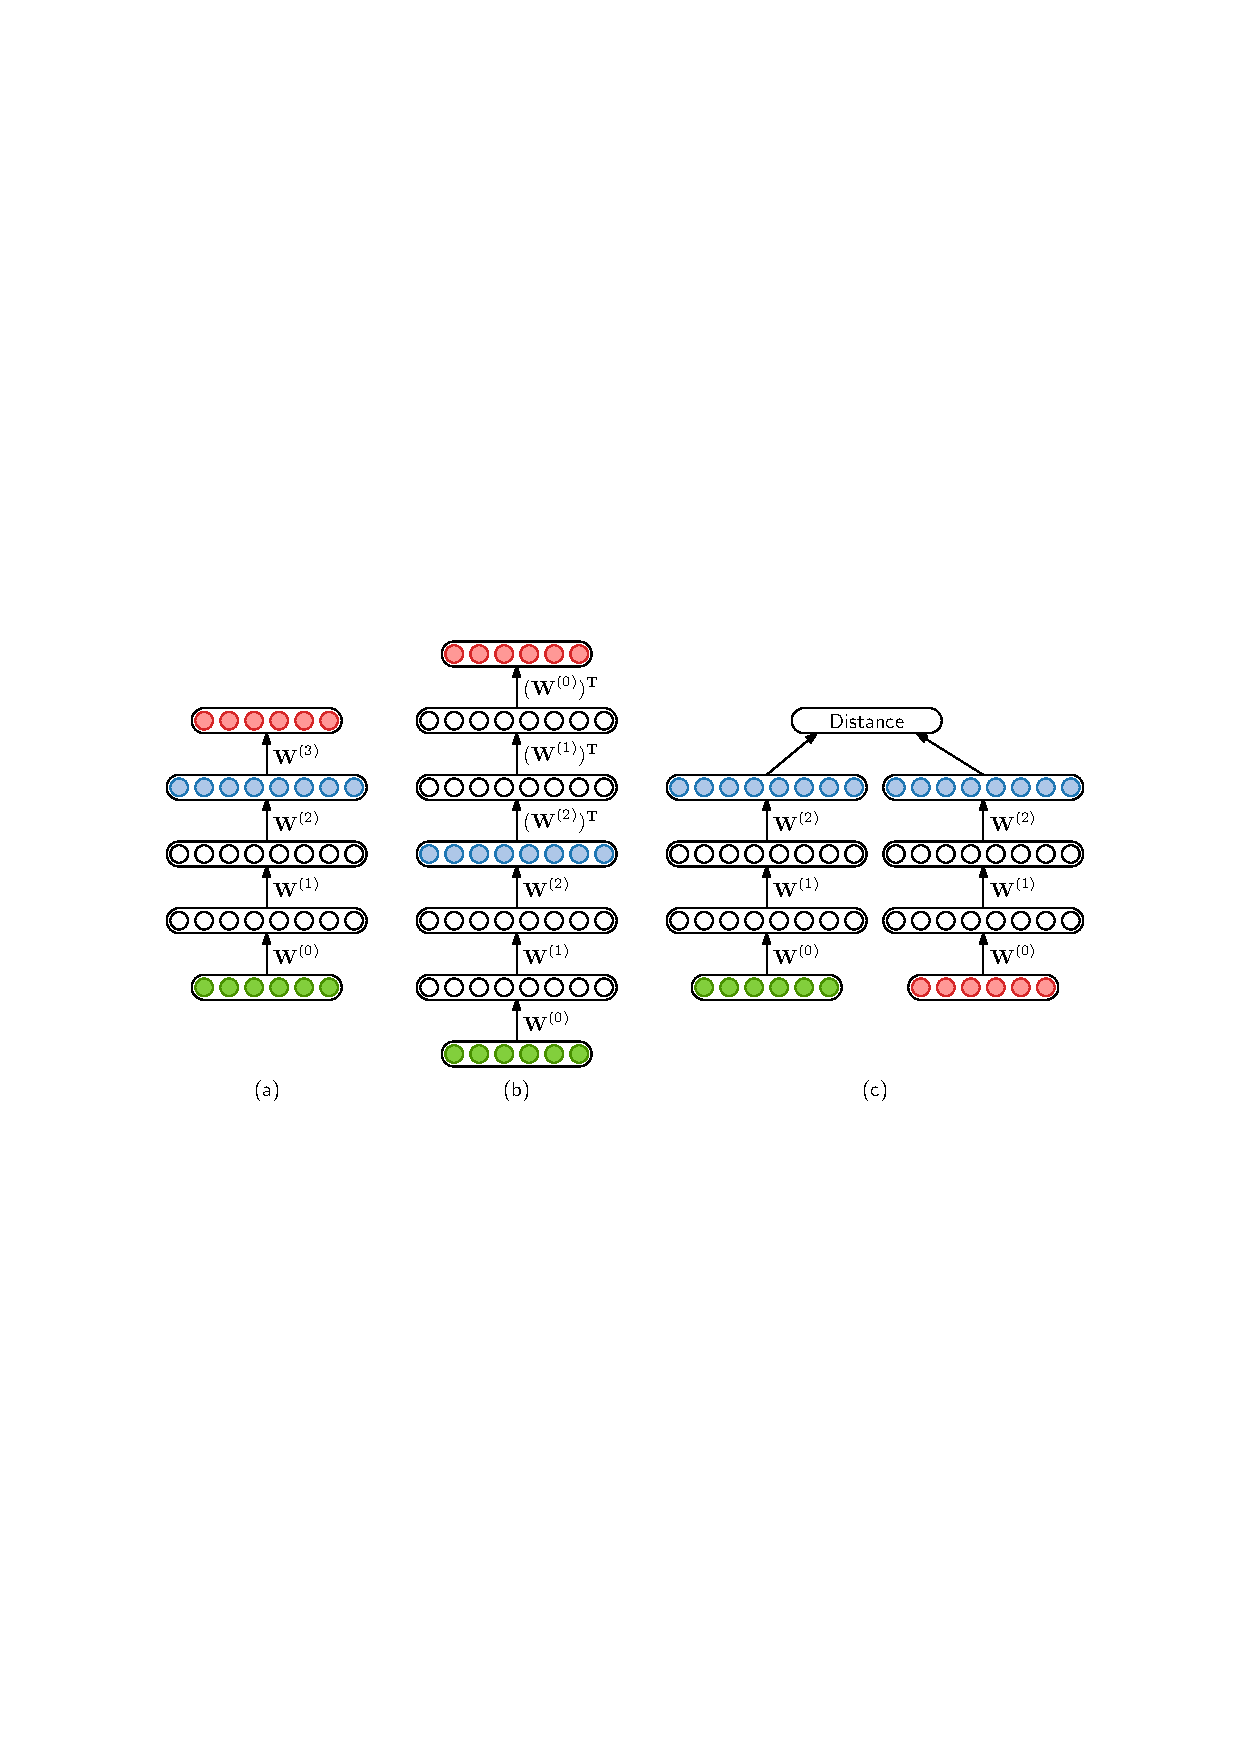
\includegraphics[width=\linewidth]{cae_siamese}
    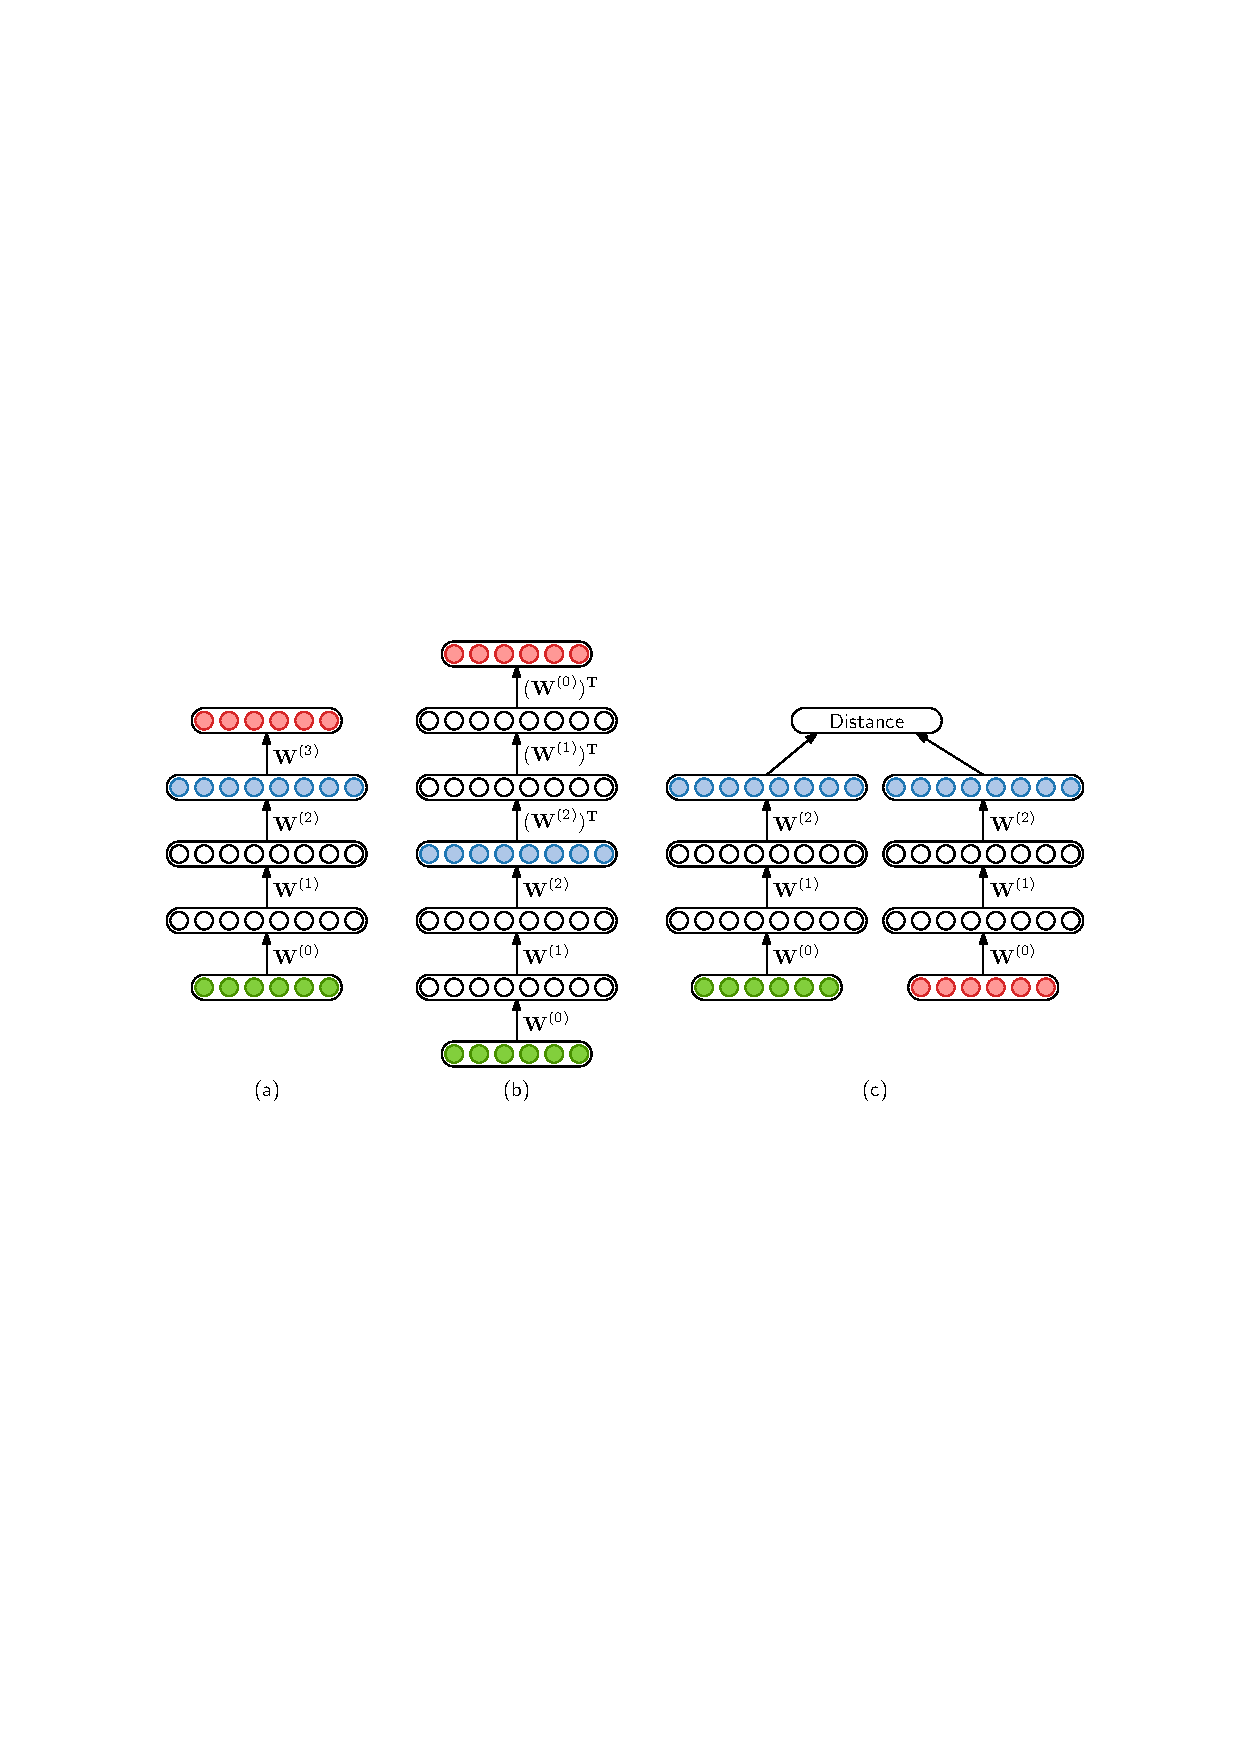
\includegraphics[width=0.918\linewidth]{cae_siamese}
    \caption[I am the short caption that appears in the list of figures, without references.]{
    (a) The cAE as used in this chapter. The encoding layer (blue) is chosen based on performance on a development set.
    (b) The cAE with symmetrical tied weights. The encoding from the middle layer (blue) is always used.
    (c) The siamese DNN. The cosine distance between aligned frames (green and red) is either minimized or maximized depending on whether the frames belong to the same (discovered) word or not.
    A cAE can be seen as a type of DNN~\cite{dahl+etal_taslp12}.
    }
    \label{fig:cae_siamese}
\end{figure}


The following is an example of an equation:
\begin{equation}
P(\vec{z} | \vec{\alpha}) = \int_{\vec{\pi}} P(\vec{z} | \vec{\pi}) \, p(\vec{\pi} | \vec{\alpha}) \, \textrm{d} \vec{\pi}
= \int_{\vec{\pi}} \prod_{k = 1}^K \pi_k^{N_k} \frac{1}{B(\vec{\alpha})} \prod_{k = 1}^K \pi_k^{\alpha_k - 1} \, \textrm{d} \vec{\pi}
\label{eq:example_equation}
\end{equation}
which you can subsequently refer to as~\eqref{eq:example_equation} or Equation~\ref{eq:example_equation}.
But make sure to consistently use the one or the other (and not mix the two ways of referring to equations).
% \input{Chapter 3/ConceptualDesign.tex}
% 

\section*{Global Matchers}

Global matchers are defined as matching techniques which take the entire image as context. They vary widely in their computational efficiency and accuracy. That is, some aim to infer the rotation and translation of the image, while others aim to quickly find the most similar image. In our context, global matchers will be used for the latter purpose. Note that while they can be used for the former purpose, because they take the entire image as context, they are highly noise sensitive, and have widely different performances for different datasets and parameters. 


There are significant amounts of global matching techniques, however, to maintain scope, I will only focus on global matchers that meet the following criteria:



\begin{itemize}
    \item Computationally efficient on a CPU. More specifically, the method shall take less than 1 second to compare at least 10 images. 
    \item Initial tests, which are not shown, show the matcher to be reasonably effective at the given problem after sufficient optimization.
    \item The technique must not require any pre- or live-training.
    \item The entire image context must be both evenly captured and weighted. 





\subsection*{Local detectors and matcher conversion techniques}
Retrofitting local matching techniques to a global matching context involves computing the similarity using the amount of good matches between images. However, this method has two issues in addition to its high computational cost. Firstly, it does not inherently find features evenly across the entire image, leading to loss of full context. Secondly, each patch can have different feature densities leading to asymmetrical position weighting. To combat this, patch or grid matching is used, and the amount of matches per patch is set well below the mean amount of expected matches per patch to ensure thorough and even feature finding across the images. This method is computationally expensive, but it is the most accurate and most robust to distortions and noise. Tests will be conducted on ORB and AKAZE with BF, FLANN AND GRAPH matchers. Machine learning-based models do not have a potential to meet the time requirement, and therefore will not be tested. 

The following methods below inherently require that images are rotationally aligned. Estimating the intra-image rotation is inherently erroneous and as such the following tests inherently account for the rotational invariance of the method. 

\subsection*{Cross-correlation}
Cross-correlation is a global matching technique that compares two images by sliding one over the other and computing the similarity at each position. 

\subsection*{Histograms}  
Histograms compare images by analyzing the distribution of pixel intensities, which represents how many pixels fall into different intensity levels. This method focuses on global color and brightness information.

\subsection*{SSIM (Structural Similarity Index)}  
SSIM compares images based on luminance, contrast, and structural information. 

\subsection*{Phase Correlation}
Phase correlation is a global matching technique that compares images by analyzing the phase difference between the Fourier transforms of the images.

\subsection*{Hashing}
Hashing is a global matching technique that compares images by computing a hash value for each image and comparing the hash values.



\subsection*{Considerations}
To estimate the best match we need to have an accurate rotational estimation. This involves having sufficient features found. However, the more features found, the more computationally expensive the method becomes. Therefore, it is key to consider using the method of each stage that provides sufficient accuracy without being computationally expensive.


\subsection*{Feature Extractors}


\subsubsection*{What is a feature Extractor}
A feature extractor is a computer vision algorithm or deep-learning model that identifies and extracts key features in an image. A feature is a pixel or weight of multiple pixels that represents a highly unique and distinctive part of an image. For instance, this could be an edge between a wall and the sky. Feature extractors are characterized by a spatial coordinate and a descriptor. A descriptor is a vector which contains information about the helps it be uniquely identified again in a new image. This can include information about the size, shape, and intensity of the feature. One can also infer the scale and orientation of the feature from the descriptor. A feature extractor also commonly includes a confidence score which indicates a score of how unique and well-defined the feature is. Ultimately, a feature extractors goal is to find unique and well-defined features that can be used to develop a complex understanding of the nuances and details of an image.
\subsubsection*{Usage in this task}
In this task, feature extractors are used to extract keypoints in images. These are used for intra-image rotational and translational estimates, and matching similar images. 



feature extractors are nb bc they r iinvariant to scale rotation and transformation. As opposed to simply correlating entire image. also less computationally expensive.
https://baotramduong.medium.com/feature-extraction-in-computer-vision-using-python-358d7c9863cb



common feature extraction techniques include edge detection, color histograms, and texture analysis



\section{Choosing a Feature Extractor}
When selecting a feature extractor, several critical factors must be considered:
\begin{itemize}
    \item \textbf{Accuracy:} The extractor needs to be accurate to ensure GPS inference is accurate. That is, the extractor should provide a sufficient quality and quantity of keypoints. This is quantified as subtending over 500 good matches from similar image pairs. 
    \item \textbf{Speed:} Be capable of real-time processing to ensure timely navigation and decision-making in dynamic environments. Specifically, initial tests must extract features in less than 1 second on a CPU. For the neural network-based models, the time taken to extract features must be less than 3 second on a CPU since they may be implemented with a GPU and CUDA libraries to improve performance. 
    \item \textbf{Robustness:} The feature extractor should exhibit invariance to changes in scale, rotation, illumination, perspective and noise to ensure accurate and repeatable performance across different flight datasets and conditions.
\end{itemize}

Feature extractors have different parameters trading-off accuracy and speed. For example, there are detection thresholds, descriptor sizes, and keypoint densities that can be adjusted to optimize performance. 

\section{Types of Feature Extractors}
\subsection{Traditional Feature Extractors}
\subsubsection{SIFT (Scale-Invariant Feature Transform)}
SIFT detects and describes local features in images. It is robust to changes in scale, rotation, and illumination, making it a reliable choice for many applications. However, its computational intensity can be a drawback in real-time scenarios.
\begin{itemize}
    \item \textbf{Advantages:} High accuracy and robustness due to its multi-scale approach and precise keypoint localization. SIFT's descriptors are highly distinctive, enabling reliable matching across different views and conditions.
    \item \textbf{Disadvantages:} High computational cost and slower processing speed due to the extensive keypoint detection and descriptor computation steps, making it less suitable for real-time applications.
\end{itemize}


\subsubsection{SURF (Speeded-Up Robust Features)}
SURF is a faster alternative to SIFT, utilizing integral images for rapid computation of image convolutions. It offers good accuracy and robustness while being computationally more efficient than SIFT.
\begin{itemize}
    \item \textbf{Advantages:} Faster than SIFT due to its use of Haar wavelets and integral images, providing good balance between speed and accuracy. It maintains robustness to scale and rotation changes.
    \item \textbf{Disadvantages:} Still relatively computationally expensive compared to simpler methods like ORB, and can be less accurate than SIFT in certain complex scenarios.
\end{itemize}



\subsubsection{ORB (Oriented FAST and Rotated BRIEF)}
ORB combines the FAST keypoint detector and the BRIEF descriptor, providing a highly efficient feature extraction method suitable for real-time applications. It is designed to be both fast and invariant to rotation and scale.
\begin{itemize}
    \item \textbf{Advantages:} High speed and efficiency, making it suitable for real-time applications. ORB's binary descriptors are computationally less intensive while providing sufficient discriminative power for many tasks.
    \item \textbf{Disadvantages:} Lower accuracy compared to SIFT and SURF, especially in complex scenes with significant variations in lighting and scale. The binary nature of BRIEF descriptors can sometimes lead to higher false match rates.
\end{itemize}

\subsection{AKAZE (Accelerated-Keypoint-Affine-Zernike)}
AKAZE is a feature extraction method that combines speed and accuracy by using nonlinear scale space and feature detection. It is designed to be robust to various transformations and lighting conditions.
\begin{itemize}
    \item \textbf{Advantages:} High speed and efficiency due to its nonlinear scale space and feature detection approach. AKAZE is robust to scale, rotation, and illumination changes, making it suitable for diverse environments.
    \item \textbf{Disadvantages:} May not be as accurate as SIFT or SURF in certain scenarios, particularly those with complex textures or repetitive patterns. The trade-off between speed and accuracy may vary depending on the application.
\end{itemize}

\subsection{Deep Learning-Based Feature Extractors}
Deep learning-based feature extractors leverage neural networks to learn feature representations directly from data. These models need to be trained on large datasets to capture complex and hierarchical features effectively. They offer high accuracy and the ability to adapt to specific tasks through transfer learning.
    \item \textbf{Advantages:} High accuracy and the ability to learn complex and hierarchical features directly from data, enabling robust performance across diverse tasks and conditions. 
    \item \textbf{Disadvantages:} Requires substantial computational resources for training and inference. The training process is data-intensive, requiring large labeled datasets to achieve optimal performance.
\end{itemize}

\subsubsection{Pre-trained Models (SuperPoint)}
Utilizing pre-trained models, like Superpoint, that are trained on large datasets are often highly accurate relative to their efficiency. They are trained on a variety of datasets and aim to generalize well to a variety of tasks.
\begin{itemize}
    \item \textbf{Advantages:} High accuracy due to extensive pre-training on large and diverse datasets. 
    \item \textbf{Disadvantages:} May not generalize well to specific datasets which are not representative of the application dataset.
\end{itemize}



\section{Evaluation for UAV-Based Navigation}
\subsection{Requirements}
For the Skripsie project, the feature extractor must meet the following initial requirements with default parameters:
\begin{itemize}
    \item 
    \item 
    \item Must be free to use and not require any pre-training or live-training. The former excludes SURF, SIFT, and the latter, deep learning-based models. 
\end{itemize}

\subsection{Recommended Feature Extractors}
The feature extractor should be applicable to application specific requirements. In the case of this project, it should be free to use and not require any pre-training or live-training due to scope. As such, the following feature extractors are recommended:
\begin{itemize}
    \item ORB: A fast and efficient feature extractor that provides a good balance between speed and accuracy. It is suitable for real-time applications and can handle scale and rotation changes effectively.
    \item AKAZE: A feature extraction method that combines speed and accuracy by using nonlinear scale space and feature detection. It is robust to various transformations and lighting conditions.
    \item SuperPoint: A pre-trained model that offers high accuracy and efficiency for real-time applications. It learns feature representations directly from data, making it adaptable to specific tasks.


    


\chapter{Results}

TESTS:
amt of keypoints for a specific runtime that are accepted as good matches
overall accuracy for heading and GPS change estimation


DATASET PARAMETERS:
image resolution vs speed accuracy
dataset terrain



All parameter choices




test 1: accuracy on a single dataset for rotational estimation (global matcher), global matching technique, and local matcher. gonna need to split those. say something about the matches are good no matter what  - not a hard task.
So test both methods (Plus neural local) on both stages (2x3 results) on a single dataset - see which is more accurate only. - total time and acc.
test 2: Take the top 3 combinations and test them on all the datasets (or as many as are close together in accuracy) - optimize for datasets - see which is more accurate only. - total time and acc. 
test 3: mess up the parameters and see how it affects the stability of different methods as well as the overall accuracy - stability, acc and time. 
test 4: test whether one performs significantly better than normally when used as the global matcher technique

XXX - note that we dont look at time per extraction as the time of latter stages is affected by the amount and quality of keypoints. So it might extract rubbish faster, but then take longer to match. So we look at total time.
Test 1 and 2 show accuracy. Test 2 and 3 show robustness. 

XXX - need to make a note on why mean heading error is not compared much - it subtends GPS error - and its estimated in this project as we dont have an accurate heading. 

XXX - say we are going to use histograms, its significantly faster, ensures no effects from the global match, could potentially test that after 







On face value, ORB has more accuracy and less time per keypoint extracted, and less total time in the most recent example. However, one also notes how the time varies significantly as the maximum number of keypoints increases. 

AKAZE has a filter threshold which is difficult to tune and highly sensitive to minor changes. Further, this threshold needs to be changed based on the dataset depending on the types of keypoints and visibility etc. As such, it is easier to use the more simple and consistent number of keypoints threshold that ORB uses. To summarize it, ORB is much easier to tune, and tends to have a higher accuracy to time ratio. To achieve the same top local minimum error, AKAZE subtends a runtime of 712 seconds, while ORB subtends a runtime of 271 seconds. This is a significant difference. 

However, AKAZE is significantly more accurate at the same time to run and time per keypoint extracted. It is also more robust to changes in the dataset. Further, a change in time does not subtend a large change in accuracy. However, AKAZE extracts much less, and higher quality keypoints. This is advantageous for efficiency and accuracy, however, it makes AKAZE highly volatile to varying datasets as it will often not acquire sufficient keypoints. This can be mitigated by having an adaptive good match filtering threshold (this is implemented). However, the AKAZE threshold still needs to be manually tuned, this can also be made dynamic, at a time cost for constant re-estimation. 

However, when trying different data sets etc - and perhaps when trying it with the local matcher, robustness might affect these end results. 





NOTE ORB simply does not work on the desert dataset 





Please note that these tests are run without optimal settings - i.e. for debug purposes certain parts run which normally would not. 




TEST 1:
Heading estimation error too high.
Heading estimation error too high.
Linear regression inferred factor x: 3.207310914993286
Linear regression inferred factor y: 3.526571035385132 

Heading estimation error too high.
Heading estimation error too high.
Heading estimation error too high.
Heading estimation error too high.
Stability analysis mean (relative to src - best result) and var*10e6
Phase Correlation stability: 1.159 +/- 68807.336
Linear Algebra stability: 1.000 +/- 56.929
Affine stability: 1.020 +/- 921.300
Rigid stability: 0.995 +/- 160.067
Homography stability: 1.108 +/- 5592.924

Percentage Deviation: [3.22100261] %
Preprocessing Global Detector: ORB, Preprocessing Global Matcher: BF, Global Matching Technique: Histogram, Local Detector: ORB, Local Matcher: BF
Mean normalized GPS error: [24.86177763]
 Mean Heading Error: 1.9734131972502695
Mean Length of Global Keypoints: 5426.8
Mean Length of Local Keypoints: 5426.8
Mean Global Time to Extract Keypoints: 0.0295 s
Mean Number of Good Matches: 604.5387931034483
Range of Good Matches: 7310
Time taken to execute The Method: 57.5468 seconds



END 1

Heading estimation error too high.
Heading estimation error too high.
Linear regression inferred factor x: 3.2284045219421387
Linear regression inferred factor y: 3.480206251144409

Heading estimation error too high.
Heading estimation error too high.
Heading estimation error too high.
Heading estimation error too high.
Stability analysis mean (relative to src - best result) and var*10e6
Phase Correlation stability: 1.163 +/- 68807.336
Linear Algebra stability: 1.000 +/- 43.544
Affine stability: 1.026 +/- 595.532
Rigid stability: 0.994 +/- 195.841
Homography stability: 1.111 +/- 5592.908

Percentage Deviation: [3.11905048] %
Preprocessing Global Detector: ORB, Preprocessing Global Matcher: BF, Global Matching Technique: Histogram, Local Detector: AKAZE, Local Matcher: BF
Mean normalized GPS error: [24.07484528]
 Mean Heading Error: 1.9734131972502695
Mean Length of Global Keypoints: 5426.8
Mean Length of Local Keypoints: 9987.666666666666
Mean Global Time to Extract Keypoints: 0.0337 s
Mean Number of Good Matches: 604.5387931034483
Range of Good Matches: 7310
Time taken to execute The Method: 67.8058 seconds


END 2

Stability analysis mean (relative to src - best result) and var*10e6
Phase Correlation stability: 1.190 +/- 68807.336
Linear Algebra stability: 1.000 +/- 176.334
Affine stability: 1.101 +/- 2279.378
Rigid stability: 0.989 +/- 473.279
Homography stability: 1.141 +/- 5715.823

Percentage Deviation: [2.75680053] %
Preprocessing Global Detector: ORB, Preprocessing Global Matcher: BF, Global Matching Technique: Histogram, Local Detector: SUPERPOINT, Local Matcher: LightGlue
Mean normalized GPS error: [21.27876627]
 Mean Heading Error: 1.9734131972502695
Type: Numpy Array
Shape: torch.Size([1, 1000, 2])
Mean Length of Global Keypoints: 5426.8
Mean Length of Local Keypoints: 1000.0
Range of Local kp: 0
Mean Global Time to Extract Keypoints: 0.0342 s
Mean Number of Glob good Matches: 604.5387931034483
Time taken to execute The Method: 130.9345 seconds

Note that superpoint and Lightglue have various tunable parameters. However, there is no way to reduce the time taken to extract and match keypoints to the point of the algorithmic models without significantly reducing accuracy. However, these models are significantly faster on GPU's and CUDA libraries. There is a decent range where one can increase time cost and gain a reasonable increase in accuracy. Superpoint and LightGLue parameters are relatively hard to tune, as there are many. However, XXX, its yet to be seen how robust these parameters are to different datasets. 

END 3


Heading estimation error too high.
Stability analysis mean (relative to src - best result) and var*10e6
Phase Correlation stability: 0.877 +/- 70819.259
Linear Algebra stability: 1.000 +/- 62.694
Affine stability: 0.998 +/- 1355.790
Rigid stability: 0.987 +/- 181.514
Homography stability: 1.044 +/- 6260.942

Percentage Deviation: [3.05771815] %
Preprocessing Global Detector: AKAZE, Preprocessing Global Matcher: BF, Global Matching Technique: Histogram, Local Detector: ORB, Local Matcher: BF
Mean normalized GPS error: [20.64342049]
 Mean Heading Error: 1.7089258086216432
Mean Length of Global Keypoints: 55.53333333333333
Mean Length of Local Keypoints: 5426.8
Range of Local kp: 7310
Mean Global Time to Extract Keypoints: 0.2273 s
Mean Number of Glob good Matches: 300.0
Time taken to execute The Method: 26.1905 seconds


END 4


Stability analysis mean (relative to src - best result) and var*10e6
Phase Correlation stability: 0.905 +/- 70819.259
Linear Algebra stability: 1.000 +/- 166.490
Affine stability: 1.044 +/- 2069.720
Rigid stability: 0.983 +/- 324.556
Homography stability: 1.077 +/- 6339.018

Percentage Deviation: [2.77759658] %
Preprocessing Global Detector: AKAZE, Preprocessing Global Matcher: BF, Global Matching Technique: Histogram, Local Detector: SUPERPOINT, Local Matcher: LightGlue
Mean normalized GPS error: [18.75224969]
 Mean Heading Error: 1.7089258086216432
Mean Length of Global Keypoints: 55.53333333333333
Mean Length of Local Keypoints: 1000.0
Range of Local kp: 0
Mean Global Time to Extract Keypoints: 0.2408 s
Mean Number of Glob good Matches: 300.0
Time taken to execute The Method: 77.1795 seconds

END 5








Another note, this data is run in debug mode, with many methods running sequentially instead of a single method. Further, this is ran in a high accuracy mode for both, with an aim to get good results for both while keeping the time between methods reasonably similar without moving far off optimal points. 








ADDITIONAL TEST:
Percentage Deviation: [2.65627788] %
Preprocessing Global Detector: AKAZE, Preprocessing Global Matcher: BF, Global Matching Technique: Histogram, Local Detector: AKAZE, Local Matcher: BF
Mean normalized GPS error: [18.24802137]
 Mean Heading Error: 1.545597672500035
Mean Length of Global Keypoints: 4083.133333333333
Mean Length of Local Keypoints: 15055.266666666666
Range of Local kp: 12695
Mean Global Time to Extract Keypoints: 0.2440 s
Mean Number of Glob good Matches: 300.0
Time taken to execute The Method: 113.2767 seconds
with akaze 0.00017, and 0.00007 for local. 



akaze akaze:
Phase Correlation stability: 0.902 +/- 46811.385
Linear Algebra stability: 1.000 +/- 38.748
Affine stability: 1.023 +/- 805.875
Rigid stability: 0.986 +/- 202.970
Homography stability: 1.114 +/- 5841.347

Percentage Deviation: [2.80564334] %
Preprocessing Global Detector: AKAZE, Preprocessing Global Matcher: BF, Global Matching Technique: Histogram, Local Detector: AKAZE, Local Matcher: BF
Mean normalized GPS error: [19.27412787]
 Mean Heading Error: 1.6004082453122863
Mean Length of Global Keypoints: 1296.9333333333334
Mean Length of Local Keypoints: 15055.266666666666
Range of Local kp: 12695
Mean Global Time to Extract Keypoints: 0.2092 s
Mean Number of Glob good Matches: 300.0
Time taken to execute The Method: 56.3528 seconds


akaze orb (local):
XXX make note abt dynamic adjustment 

% \input{Chapter 4/Methodology.tex}
\chapter{Comparison of Methods}



\section{Testing Setup}

This section outlines the framework used to evaluate the performance of the proposed UAV navigation methods. The evaluation focuses on three primary metrics: accuracy, runtime, and robustness. These metrics are critical to ensure that the navigation system can reliably operate under diverse and challenging conditions, reflecting real-world scenarios where the UAV may encounter varying environmental factors.

\subsection{Datasets}

Five distinct datasets were selected to comprehensively test the methods' ability to generalize and perform in different environments:

\begin{itemize}
    \item \textbf{CITY1 and CITY2} (Cape Town): Both datasets originate from Cape Town. CITY1 incorporates both rotational and translational changes between frames, while CITY2 includes only translational changes. This distinction allows for the isolation of performance under rotational loads.
    \item \textbf{ROCKY}: Represents rugged terrain with varied features, testing the methods' ability to handle complex topographies.
    \item \textbf{DESERT and AMAZON}: Characterized by extreme sparsity and repetitive patterns, these datasets present significant challenges even for human observers to distinguish differences.
\end{itemize}


\subsection{Testing Structure}

Each method, including feature extraction, local feature matching, rotational estimation, image similarity computation, translational estimation, and optimization techniques, is subjected to rigorous testing based on the following criteria:

\begin{itemize}
    \item \textbf{Accuracy}: Evaluated using the Root Mean Square Error (RMSE) of GPS estimations, accuracy assessments focus on the end error. This is justified because outputs—whether images or degrees—propagate through the pipeline, meaning any errors or poor choices are ultimately reflected in the final GPS error.
    \item \textbf{Accuracy}: Evaluated using the Root Mean Square Error (RMSE) of GPS estimations, accuracy assessments focus on the end error. This approach is preferable because intermediate outputs do not always provide clear indicators of quality. For instance, the number of keypoints can be misleading; without context, it's difficult to determine if they represent good features or excessive noise. Outputs propagate through the pipeline, meaning any errors or poor choices are ultimately reflected in the final GPS error, making it more effective to measure accuracy at the end.
    \item \textbf{Runtime}: The entire system runtime per dataset is assessed to evaluate the computational efficiency of each method. Efficient runtimes are crucial for real-time UAV applications, as delays—combined with pilot and UAV response times—can result in consistently missing the target and failing to follow the intended path. As before, runtime may propagate through the system, and therefore the runtime per line is not necessarily indicative of better performance; Runtime per line is not tested. 
    \item \textbf{Robustness}: Tested to verify each method's stability under parameter variations and challenging conditions. Robust methods maintain consistent performance despite environmental or parameter changes, ensuring reliable UAV navigation across different scenarios.
\end{itemize}

This structured testing approach ensures that each component of the UAV navigation system is thoroughly evaluated, facilitating the selection of methods that deliver optimal performance across all critical metrics.

\subsection{Parameters}  
Parameters were held constant across tests and chosen to ensure optimal performance across methods. The focus was not on selecting the absolute best parameter set, as this was not relevant for inter-method testing; rather, the goal was to minimize bias while allowing each method to perform effectively. For instance, multiple methods were tested within a single runtime to enhance testing speed without compromising the integrity of the inter-method comparisons. The takeaway here is to avoid interpreting results objectively, as they do not reflect the realistic and overall performance of the system.



\section{Feature Detectors}

This section presents the evaluation results of three feature detectors: ORB, AKAZE, and SuperPoint with LightGlue. The primary objective of this evaluation is to identify the most suitable detector for a UAV navigation system tasked with estimating rotational and translational transformations. Key performance metrics, including RMSE (Root Mean Square Error), runtime, and robustness across multiple datasets, were considered to assess each detector's effectiveness and suitability.

\subsection{Testing Overview}

The feature detectors were assessed based on their ability to accurately estimate transformations under various conditions. Consistent parameters were maintained across all datasets to ensure a fair comparison. Notably, AKAZE lacked a built-in keypoint target parameter, resulting in highly variable runtimes across datasets due to the necessity of selecting a parameter that identified sufficient keypoints for each dataset. To address this variability, dynamic thresholding was implemented for AKAZE, enabling keypoint target thresholds comparable to those of the other detectors.

The evaluation focused on three main criteria:
\begin{itemize}
    \item \textbf{Accuracy (RMSE in GPS)}: Measures the precision of transformation estimates.
    \item \textbf{Runtime}: Assesses the computational efficiency of each detector.
    \item \textbf{Robustness}: Evaluates consistency and reliability across different datasets.
\end{itemize}

The results from these tests informed the selection of the most appropriate detector and threshold parameters for the four defined stages utilizing the detected keypoints: rotational alignment for global matching, global similarity computation, precise translation estimation, and precise rotational estimation.

\subsection{Translation Estimation Performance}

Table \ref{tab:rmse_detectors} presents the RMSE values in meters for each feature detector applied to the precise translation estimation stage. AKAZE, utilizing dynamic keypoint targeting, demonstrated the highest accuracy across all datasets while maintaining reasonable runtime. ORB exhibited respectable accuracy but was consistently outperformed by AKAZE. SuperPoint recorded the highest RMSE values, particularly in challenging datasets such as ROCKY and AMAZON, indicating its limited generalizability across diverse environments.

\begin{table}[H]
    \centering
    \caption{RMSE for Various Local Detectors (in meters)}
    \label{tab:rmse_detectors}
    \begin{tabular}{|c|c|c|c|c|c|}
    \hline
    \textbf{Method} & \textbf{CITY1} & \textbf{CITY2} & \textbf{ROCKY} & \textbf{DESERT} & \textbf{AMAZON} \\ \hline
    ORB & 70.89 & 10.56 & 43.32 & 80.66 & 46.39 \\ \hline
    \makecell{\textbf{Dynamic AKAZE} \\ \textbf{(3000 keypoints)}} & 66.80 & 6.91 & 22.48 & 33.07 & 39.27 \\ \hline
    SuperPoint & 72.66 & 15.80 & 114.93 & 31.60 & 329.19 \\ \hline
    \end{tabular}
\end{table}

\subsubsection*{Runtime and Efficiency}

Table \ref{tab:runtime_detectors} illustrates the runtime (in seconds) for each feature detector across different datasets. ORB proved to be the most efficient detector, making it suitable for applications requiring fast processing. Dynamic AKAZE, while exhibiting longer runtimes, achieved a balance between efficiency and accuracy. SuperPoint demonstrated the longest runtimes across all datasets, highlighting its limited applicability for time-sensitive applications unless optimized with GPU acceleration.

\begin{table}[H]
    \centering
    \caption{Runtime for Various Local Detectors (in seconds)}
    \label{tab:runtime_detectors}
    \begin{tabular}{|c|c|c|c|c|c|}
    \hline
    \textbf{Method} & \textbf{CITY1} & \textbf{CITY2} & \textbf{ROCKY} & \textbf{DESERT} & \textbf{AMAZON} \\ \hline
    ORB & 75.25 & 70.77 & 111.64 & 58.29 & 75.34 \\ \hline
    \makecell{\textbf{Dynamic AKAZE} \\ \textbf{(3000 keypoints)}} & 112.18 & 104.16 & 127.86 & 108.86 & 119.76 \\ \hline
    SuperPoint & 338.21 & 292.11 & 307.93 & 277.73 & 291.01 \\ \hline
    \end{tabular}
\end{table}

\subsubsection*{Robustness}

In terms of robustness, AKAZE exhibited the highest consistency in accuracy across different datasets. ORB also performed well but showed greater variability in accuracy across datasets compared to AKAZE. SuperPoint, however, demonstrated significant performance variability, indicating lower robustness across diverse environments.

\subsection{Rotation Estimation Performance}

Table \ref{tab:rmse_rot_comparison} presents the RMSE values in meters for ORB and AKAZE applied to the precise rotational estimation stage. Both detectors were optimized for this stage to ensure high accuracy while maintaining reasonable runtime.

\begin{table}[H]
    \centering
    \caption{RMSE for ORB (8000 keypoints) and AKAZE (6000 keypoints) (in meters)}
    \label{tab:rmse_rot_comparison}
    \begin{tabular}{|c|c|c|c|c|c|}
    \hline
    \textbf{Method} & \textbf{CITY1} & \textbf{CITY2} & \textbf{ROCKY} & \textbf{DESERT} & \textbf{AMAZON} \\ \hline
    ORB (8000 keypoints) & 69.42 & 8.17 & 22.38 & 32.55 & 37.93 \\ \hline
    \makecell{\textbf{Dynamic AKAZE} \\ \textbf{(6000 keypoints)}} & 68.14 & 8.34 & 21.72 & 35.17 & 39.25 \\ \hline
    \end{tabular}
\end{table}

\subsubsection*{Runtime and Efficiency}

Table \ref{tab:runtime_comparison_rot} presents the runtime comparisons for ORB and AKAZE in the rotational estimation stage. ORB outperformed AKAZE in terms of speed, especially in denser datasets, while maintaining similar levels of accuracy. This suggests that ORB is better suited for time-sensitive applications within this stage.

\begin{table}[H]
    \centering
    \caption{Runtime for ORB (8000 keypoints) and AKAZE (6000 keypoints) (in seconds)}
    \label{tab:runtime_comparison_rot}
    \begin{tabular}{|c|c|c|c|c|c|}
    \hline
    \textbf{Method} & \textbf{CITY1} & \textbf{CITY2} & \textbf{ROCKY} & \textbf{DESERT} & \textbf{AMAZON} \\ \hline
    ORB (8000 keypoints) & 95.80 & 106.63 & 104.79 & 99.56 & 84.70 \\ \hline
    \makecell{\textbf{Dynamic AKAZE} \\ \textbf{(6000 keypoints)}} & 108.44 & 131.10 & 120.77 & 111.25 & 98.70 \\ \hline
    \end{tabular}
\end{table}

\subsubsection*{Robustness}

Regarding robustness, AKAZE demonstrated more consistent accuracy across various datasets compared to ORB, which exhibited greater variability in performance. Despite this, ORB's consistently lower runtimes make it a favorable option for applications where speed is critical.

\subsection{Final Selection of Feature Detectors}

Based on the comprehensive evaluation, the following detectors were selected for the respective stages of the UAV navigation system:

\begin{itemize}
    \item \textbf{Translation Estimation Stage:} 
    AKAZE, with dynamic keypoint targeting (3000 keypoints), exhibited the highest accuracy and robustness in translation estimation while maintaining reasonable runtime. This balance makes Dynamic AKAZE the optimal choice for precise translation inference.
    
    \item \textbf{Rotational Alignment for Translation Estimation Stage:} 
    ORB, utilizing 8000 keypoints, offers an excellent balance between accuracy and efficiency. Although AKAZE demonstrated slightly better performance in rotational estimation, ORB's significantly lower runtime makes it the preferred option for this stage.
    
    \item \textbf{Rotational Alignment for Global Matching Stage:} 
    ORB, with 6000 keypoints, is the optimal choice due to its superior runtime efficiency. This stage can accommodate relatively larger rotational estimation errors, making ORB ideal for global matching tasks.
    
    \item \textbf{Global Similarity Refinement:} 
    ORB, employing 1500 keypoints, is selected for global image similarity comparison using local matching. The lower accuracy requirement and the necessity for high runtime efficiency make ORB the best fit for grid matching.
\end{itemize}

These selections ensure that each stage of the UAV navigation system leverages the most appropriate feature detector, optimizing both accuracy and computational performance.



\section{Local Feature Matchers}

This section evaluates two prominent local matchers, BFMatcher and FLANN, within the context of a UAV navigation system. The primary objective of this evaluation is to determine the most efficient and robust matcher in terms of accuracy, runtime, and consistency across diverse datasets. These matchers play a crucial role in the system's ability to accurately estimate rotational and translational transformations by effectively pairing detected feature points.

\subsection{Testing Overview}

The local matchers were assessed under various conditions to evaluate their performance concerning accuracy (RMSE in GPS), runtime, and robustness. The evaluation was meticulously designed to understand how each matcher handles noisy keypoints, limited post-match filtering, and varying detector thresholds. The goal was to identify which matcher offers the most suitable balance between match quality and computational efficiency, thereby ensuring real-time applicability in UAV navigation.

\subsection{Accuracy Evaluation}

Table \ref{tab:flann_bf_comparison_acc} presents the Root Mean Squared Error (RMSE) in GPS values for BFMatcher and FLANN across different datasets. The results indicate that while BFMatcher achieves slightly better accuracy in certain cases, FLANN remains highly competitive with only marginally higher RMSE values.

\begin{table}[H]
    \centering
    \caption{RMSE GPS Accuracy for BFMatcher and FLANN (in meters)}
    \label{tab:flann_bf_comparison_acc}
    \begin{tabular}{|c|c|c|c|c|c|}
    \hline
    \textbf{Matcher} & \textbf{CITY1} & \textbf{CITY2} & \textbf{ROCKY} & \textbf{DESERT} & \textbf{AMAZON} \\ \hline
    FLANN          & 56.59           & 4.70           & 14.63          & 71.20           & 32.35           \\ \hline
    BFMatcher      & 53.89           & 3.79           & 16.36          & 68.64           & 33.24           \\ \hline
    \end{tabular}
\end{table}

\textbf{Observations:}
\begin{itemize}
    \item \textbf{BFMatcher Accuracy:} BFMatcher demonstrated slightly superior accuracy in CITY1 and CITY2 compared to FLANN. However, the improvement was not substantial enough to outweigh its increased computational demands.
    \item \textbf{FLANN Accuracy:} FLANN maintained competitive accuracy levels, trailing BFMatcher only marginally in most datasets. Notably, FLANN exhibited strong performance in the ROCKY dataset, underscoring its reliability in challenging environments.
\end{itemize}

\subsection{Runtime Evaluation}

Table \ref{tab:flann_bf_comparison_runtime} illustrates the runtime (in seconds) for BFMatcher and FLANN across different datasets. The results clearly show that FLANN consistently outperforms BFMatcher in terms of speed, with significantly lower execution times across all datasets.

\begin{table}[H]
    \centering
    \caption{Runtime Comparison for BFMatcher and FLANN (in seconds)}
    \label{tab:flann_bf_comparison_runtime}
    \begin{tabular}{|c|c|c|c|c|c|}
    \hline
    \textbf{Matcher} & \textbf{CITY1} & \textbf{CITY2} & \textbf{ROCKY} & \textbf{DESERT} & \textbf{AMAZON} \\ \hline
    FLANN          & 42.72           & 41.61          & 41.96          & 43.42           & 53.62           \\ \hline
    BFMatcher      & 203.49          & 228.59         & 46.33          & 52.59           & 88.95           \\ \hline
    \end{tabular}
\end{table}

\textbf{Observations:}
\begin{itemize}
    \item \textbf{FLANN Efficiency:} FLANN exhibited significantly faster runtimes across all datasets, particularly excelling in CITY1 and CITY2 where it completed tasks in less than a quarter of the time required by BFMatcher.
    \item \textbf{BFMatcher Runtime:} The exhaustive matching approach of BFMatcher resulted in considerably higher runtimes, rendering it less suitable for real-time applications where speed is critical.
\end{itemize}

\subsection{Robustness Under Varying Detector Thresholds}

Figure \ref{fig:divergence_plot} depicts the divergence in RMSE GPS error between FLANN and BFMatcher as the number of keypoints increases. Positive values indicate that BFMatcher outperforms FLANN, while negative values suggest FLANN performs better.

\begin{figure}[H]
    \centering
    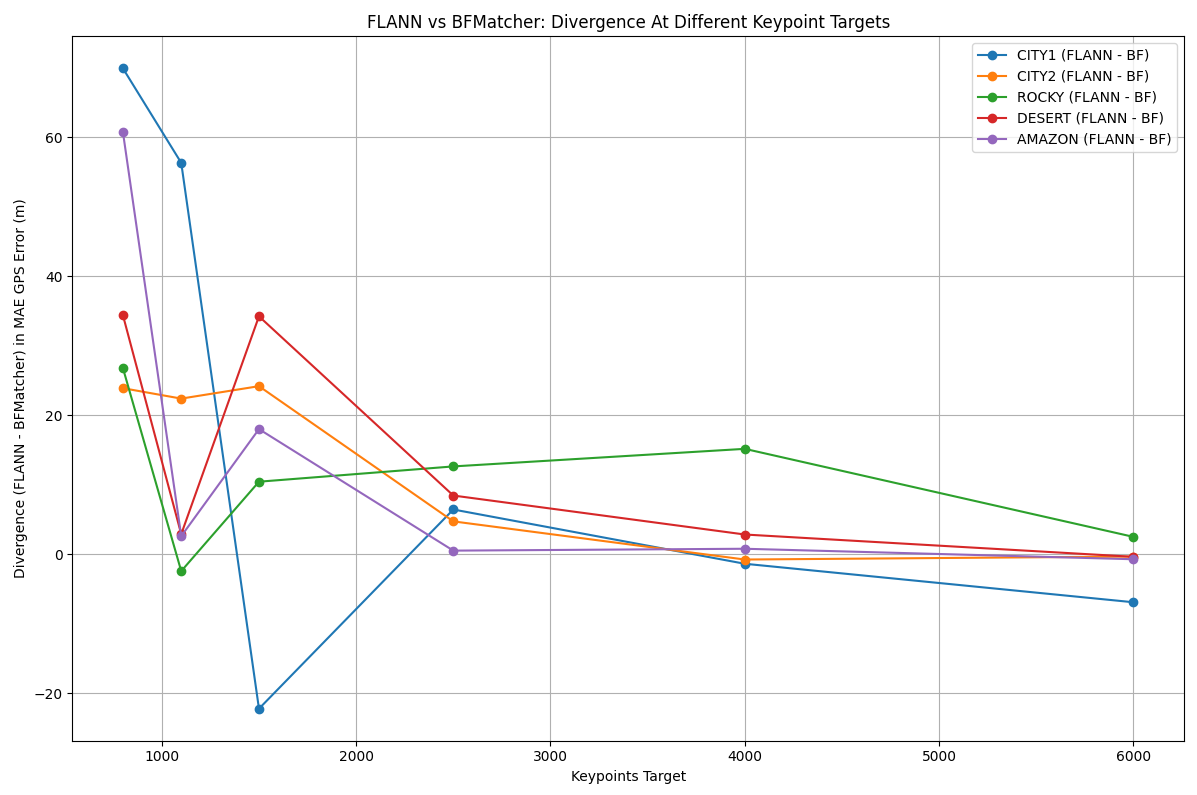
\includegraphics[width=\textwidth]{./Graphs/Divergence_BF_FLANN_KPS.png}
    \caption{Divergence in RMSE GPS Error Between FLANN and BFMatcher Across Keypoint Targets}
    \label{fig:divergence_plot}
\end{figure}

\textbf{Observations:}
\begin{itemize}
    \item \textbf{Convergence:} Both matchers demonstrated similar accuracy levels as the number of keypoints increased, with performance becoming nearly identical beyond 2500 keypoints. Given that feature detectors are typically configured with a keypoint target of at least 3000, both matchers are expected to perform comparably in standard operational conditions.
    \item \textbf{Outliers:} Although BFMatcher generally outperforms FLANN, there are instances where FLANN achieves better accuracy. This can occur due to FLANN’s approximate matching, which may preserve valid matches that BFMatcher might discard using Lowe’s ratio thresholding.
    \item \textbf{Scalability:} FLANN's runtime scalability with increasing keypoint counts was superior to that of BFMatcher, making FLANN a more scalable solution for larger datasets.
\end{itemize}

\subsection{Final Selection of Local Feature Matcher}

Based on the comprehensive evaluation of accuracy, runtime, and robustness, FLANN emerges as the optimal choice for the UAV navigation system. FLANN offers significantly faster runtimes and better scalability while maintaining comparable accuracy to BFMatcher. This makes FLANN highly suitable for real-time applications where computational efficiency is paramount.

\begin{itemize}
    \item \textbf{Overall Choice:} \textbf{FLANN} is selected as the primary local feature matcher for the UAV navigation system, balancing high performance and efficiency across diverse operational conditions.
\end{itemize}

These selections ensure that the UAV navigation system leverages the most appropriate local matcher, optimizing both accuracy and computational performance to achieve reliable and efficient navigation.


\section{Rotational Estimators}

This section evaluates the performance of three rotational estimation methods: Partial Affine 2D, Affine 2D, and Homography. The objective is to identify the most suitable method for UAV navigation by comparing accuracy, runtime, and robustness across various datasets. These estimators are critical for accurately determining the rotational transformations required for precise navigation and alignment of UAV imagery.

\subsection{Testing Overview}

The rotational estimators were assessed based on their ability to accurately estimate rotations under diverse conditions. Consistent parameters were maintained across all datasets to ensure a fair comparison. The evaluation focused on three primary criteria:
\begin{itemize}
    \item \textbf{Accuracy (RMSE in GPS)}: Measures the precision of rotational estimates.
    \item \textbf{Runtime}: Assesses the computational efficiency of each estimator.
    \item \textbf{Robustness}: Evaluates the consistency and reliability of each method across different datasets.
\end{itemize}

Additionally, an improvement technique involving the application of a rigid transform using Singular Value Decomposition (SVD) was explored. Although initially less effective as a standalone method, the rigid transform consistently enhanced overall accuracy when applied after other estimation methods.

\subsection{Accuracy Evaluation}

Root Mean Square Error (RMSE) was utilized to evaluate the estimation error of each method across five datasets. Table \ref{tab:rmse_comparison_rotestim} summarizes the RMSE values (in meters) for Partial Affine 2D, Affine 2D, and Homography.

\begin{table}[H]
    \centering
    \caption{RMSE Comparison Across Datasets for Partial Affine 2D, Affine 2D, and Homography}
    \label{tab:rmse_comparison_rotestim}
    \begin{tabular}{|c|c|c|c|}
    \hline
    \textbf{Dataset} & \textbf{Partial Affine 2D} & \textbf{Affine 2D} & \textbf{Homography} \\ \hline
    CITY1   & 70.18 & 81.22 & 76.25 \\ \hline
    CITY2   & 7.54  & 7.80  & 7.16  \\ \hline
    ROCKY   & 27.98 & 22.10 & 24.40 \\ \hline
    DESERT  & 44.94 & 43.11 & 48.56 \\ \hline
    AMAZON  & 46.98 & 52.56 & 48.04 \\ \hline
    \end{tabular}
\end{table}

\textbf{Observations:}  
\begin{itemize}
    \item \textbf{Partial Affine 2D Accuracy:} Partial Affine 2D exhibited the lowest combined normalized RMSE across all datasets, indicating superior overall accuracy.
    \item \textbf{Affine 2D Accuracy:} Affine 2D demonstrated competitive accuracy, particularly excelling in the ROCKY dataset.
    \item \textbf{Homography Accuracy:} Homography maintained respectable accuracy but was outperformed by Partial Affine 2D in most datasets.
    \item \textbf{Dataset-Specific Performance:} The most accurate estimator varied per dataset, highlighting the importance of method selection based on specific environmental conditions.
\end{itemize}

\subsection{Runtime Evaluation}

Table \ref{tab:runtime_comparison_rotestim} presents the runtime (in seconds) for each rotational estimator across the five datasets. The results reflect the computational efficiency of each method relative to their transformation complexity.

\begin{table}[H]
    \centering
    \caption{Runtime Comparison Across Datasets for Partial Affine 2D, Affine 2D, and Homography}
    \label{tab:runtime_comparison_rotestim}
    \begin{tabular}{|c|c|c|c|}
    \hline
    \textbf{Dataset} & \textbf{Partial Affine 2D} & \textbf{Affine 2D} & \textbf{Homography} \\ \hline
    CITY1   & 56.76 & 65.27 & 68.79 \\ \hline
    CITY2   & 52.20 & 54.55 & 65.11 \\ \hline
    ROCKY   & 69.44 & 76.16 & 78.92 \\ \hline
    DESERT  & 56.40 & 71.52 & 69.97 \\ \hline
    AMAZON  & 50.34 & 58.16 & 58.27 \\ \hline
    \end{tabular}
\end{table}

\textbf{Observations:}  
\begin{itemize}
    \item \textbf{Runtime Efficiency:} Partial Affine 2D consistently demonstrated the fastest runtimes across all datasets, followed by Affine 2D and Homography.
    \item \textbf{Complexity Correlation:} The runtime generally correlated with the transformation model's complexity, with more complex models requiring longer computation times.
    \item \textbf{Dataset-Specific Efficiency:} Partial Affine 2D maintained superior efficiency even in more demanding datasets such as ROCKY and DESERT.
\end{itemize}

\subsection{Robustness Testing}

Robustness testing assessed each method's sensitivity to parameter variations, including Lowe’s ratio, RANSAC thresholds, and keypoint quantity. This evaluation was essential to determine the performance consistency of each method under different conditions. For the sake of brevity, the results are omitted; The observations are summarized below.



\textbf{Observations:}  
\begin{itemize}
    \item \textbf{Parameter Sensitivity:} All methods exhibited high robustness against parameter variations, maintaining consistent performance across different settings.
    \item \textbf{Homography Variability:} Homography showed greater variability in accuracy when fewer matches were available, attributable to the complexity of its transformation model.
    \item \textbf{Consistent Performance:} Partial Affine 2D maintained stable performance across all datasets, reinforcing its suitability for diverse environmental conditions given its simplified transformation model.
\end{itemize}

\subsection{Improvement Technique}

An additional method, the rigid transform using Singular Value Decomposition (SVD), was initially evaluated as a primary rotational estimator. However, it performed significantly worse than the other methods and was subsequently excluded from standalone consideration. Notably, when the rigid transform was applied after other estimation methods, it consistently enhanced overall accuracy. This improvement is likely due to the rigid transform's ability to make minor, precise corrections once the point cloud is largely aligned by other methods, despite its initial inefficiency in handling outliers in the case of large misalignments.

\subsection{Final Selection of Rotational Estimator}

Based on the comprehensive evaluation of accuracy, runtime, and robustness, Partial Affine 2D emerged as the most suitable primary rotational estimator for the UAV navigation system. It demonstrated the lowest combined normalized RMSE across all datasets, the fastest runtime, and high robustness. Additionally, the application of the rigid transform using SVD after Partial Affine 2D further enhanced overall accuracy, ensuring precise rotational alignment.

\section{Image Similarity Estimators}

Accurate image similarity estimation, or global matching, is essential for UAV navigation systems to choose reasonable images to compare to. They should ensure accuracy and efficiency while maintaining robustness against small rotational offsets. This section evaluates different global matching techniques across multiple datasets to identify the most suitable method for UAV navigation based on accuracy, runtime, and robustness.

\subsection{Accuracy Evaluation}

Naturally, the appropriateness of the choice of best match is implicitly passed through to subsequent stages and realized as an error in GPS estimations. Root Mean Square Error (RMSE) was utilized to assess the GPS estimation accuracy of each global matching technique across the five datasets. Table \ref{tab:RMSE_GLOBAL_MATCHING} summarizes the RMSE values (in meters) for Local Retrofit, Cross Correlation, Histogram, and SSIM.

\begin{table}[H]
    \centering
    \caption{RMSE Comparison Across Datasets for Various Global Matching Techniques (in meters)}
    \label{tab:RMSE_GLOBAL_MATCHING}
    \begin{tabular}{|c|c|c|c|c|c|}
    \hline
    \makecell{Global Matching \\ Technique} & \makecell{CITY1} & \makecell{CITY2} & \makecell{ROCKY} & \makecell{DESERT} & \makecell{AMAZON} \\ \hline
    \makecell{Local Retrofit} & 46.56 & 7.37 & 17.32 & 128.43 & 34.54 \\ \hline
    \makecell{Cross Correlation} & 49.88 & 5.12 & 15.77 & 26.84 & 31.50 \\ \hline
    Histogram & 46.35 & 5.12 & 15.77 & 27.28 & 31.50 \\ \hline
    SSIM & 50.03 & 6.16 & 15.77 & 27.28 & 31.44 \\ \hline
    \end{tabular}
\end{table}

\textbf{Observations:}  
\begin{itemize}
    \item \textbf{Histogram Accuracy:} The Histogram technique consistently achieved the lowest RMSE across most datasets, particularly excelling in CITY1, CITY2, and ROCKY.
    \item \textbf{Cross Correlation Accuracy:} Cross Correlation closely followed Histogram in accuracy, demonstrating strong performance in CITY2 and DESERT.
    \item \textbf{SSIM Accuracy:} SSIM maintained comparable accuracy to Histogram and Cross Correlation but exhibited slightly higher errors in CITY1 and DESERT.
    \item \textbf{Local Retrofit Accuracy:} The Local Retrofit method recorded the highest RMSE values, especially in the DESERT dataset, indicating poor generalizability and higher complexity. Consequently, it was excluded from further analysis.
\end{itemize}

\subsection{Runtime Evaluation}

Table \ref{tab:RUNTIME_GLOBAL_MATCHING} compares the computational efficiency of each global matching technique across the five datasets.

\begin{table}[H]
    \centering
    \caption{Runtime Comparison Across Global Matching Techniques (in seconds)}
    \label{tab:RUNTIME_GLOBAL_MATCHING}
    \begin{tabular}{|c|c|c|c|c|c|}
    \hline
    \makecell{Global Matching \\ Technique} & \makecell{CITY1} & \makecell{CITY2} & \makecell{ROCKY} & \makecell{DESERT} & \makecell{AMAZON} \\ \hline
    \makecell{Local Retrofit} & 84.56 & 76.34 & 70.22 & 63.47 & 90.69 \\ \hline
    \makecell{Cross Correlation} & 59.62 & 56.67 & 54.14 & 59.90 & 65.92 \\ \hline
    Histogram & 57.06 & 56.33 & 56.68 & 51.98 & 59.09 \\ \hline
    SSIM & 91.60 & 77.99 & 83.31 & 83.08 & 114.07 \\ \hline
    \end{tabular}
\end{table}

\textbf{Observations:}  
\begin{itemize}
    \item \textbf{Histogram Efficiency:} The Histogram technique was the most efficient in terms of runtime, outperforming all other methods consistently across all datasets.
    \item \textbf{Cross Correlation Efficiency:} Cross Correlation followed closely behind Histogram, offering slightly higher runtimes but still maintaining high computational efficiency.
    \item \textbf{SSIM Efficiency:} SSIM exhibited the longest runtimes, particularly in the AMAZON and DESERT datasets, rendering it less suitable for real-time applications.
    \item \textbf{Local Retrofit Efficiency:} The Local Retrofit method had the highest runtimes and was deemed non-viable due to its excessive computational cost and poor accuracy.
\end{itemize}

\subsection{Robustness to Rotational Offsets}

Robustness testing evaluated each global matching technique's sensitivity to a 10-degree rotational offset. All matchers that made it this far saw no change in choice combination below a 5-degree offset. The impact on RMSE GPS error and the percentage change in error were recorded to assess each method's stability under rotational misalignments.

\begin{table}[H]
    \centering
    \caption{RMSE (GPS Error) and Percentage Change with 10-degree Rotational Offset}
    \label{Robustness_GlobalMatchers}
    \begin{tabular}{|c|c|c|c|c|c|c|}
    \hline
    \textbf{Method} & \textbf{Metric} & \textbf{CITY1} & \textbf{CITY2} & \textbf{ROCKY} & \textbf{DESERT} & \textbf{AMAZON} \\ \hline
    \multirow{2}{*}{\makecell{Cross Correlation}} & RMSE & 54.81 & 5.34 & 17.55 & 32.51 & 31.52 \\ \cline{2-7}
    & \% Change & 5.89\% & 4.29\% & 11.54\% & 21.92\% & 0.06\% \\ \hline
    \multirow{2}{*}{\makecell{Histogram}} & RMSE & 56.17 & 4.45 & 16.83 & 37.20 & 36.35 \\ \cline{2-7}
    & \% Change & 20.93\% & -13.09\% & 6.73\% & 36.73\% & 15.38\% \\ \hline
    \multirow{2}{*}{\makecell{SSIM}} & RMSE & 55.93 & 5.53 & 16.25 & 41.01 & 31.67 \\ \cline{2-7}
    & \% Change & 11.79\% & -10.23\% & 3.04\% & 50.43\% & 0.73\% \\ \hline
    \end{tabular}
\end{table}

\textbf{Observations:}  
\begin{itemize}
    \item \textbf{Cross Correlation Robustness:} Cross Correlation exhibited the lowest percentage change in GPS error under a 10-degree rotational offset, indicating strong robustness.
    \item \textbf{Histogram Robustness:} While Histogram demonstrated competitive RMSE values, it showed significant deviations in the DESERT and AMAZON datasets when subjected to rotational offsets.
    \item \textbf{SSIM Robustness:} SSIM displayed higher error rates and greater variability, particularly in the DESERT dataset, making it less robust to significant rotational misalignments.
\end{itemize}

\subsection{Improvement Technique}

An additional method, the rigid transform using Singular Value Decomposition (SVD), was initially evaluated as a primary global matching technique. However, it performed significantly worse than the other methods and was subsequently excluded from standalone consideration. However, when the rigid transform was applied after other estimation methods, it consistently enhanced overall accuracy. This improvement is likely due to the rigid transform's ability to make minor, precise corrections once the point cloud is largely aligned by other methods, despite its initial inefficiency in handling large misalignments.

\subsection{Final Selection of Global Matching Technique}

Based on the comprehensive evaluation of accuracy, runtime, and robustness, the \textbf{Histogram} technique is identified and chosen as the most suitable global matching method for the system. Histogram consistently provided superior performance in terms of both RMSE and runtime, particularly under large rotational offsets. Although Cross Correlation also demonstrated strong performance, Histogram's marginally better accuracy and runtime efficiency make it the preferred choice.



\section{Translational Estimators}

This section evaluates the performance of various translational estimation methods for UAV navigation. The methods assessed include Phase Correlation, Rigid Transform, Affine Transform with RANSAC, Homography Transform, and Partial Affine 2D. Each method is evaluated based on accuracy, runtime, and robustness across multiple datasets to identify the most effective option for UAV navigation.

\subsection{Accuracy Evaluation}

Root Mean Square Error (RMSE) was utilized to assess the GPS estimation accuracy of each translational estimation method across five datasets. Table \ref{tab:rmse_comparison_transestim} summarizes the RMSE values (in meters) for each method.

\begin{table}[H]
    \centering
    \caption{RMSE GPS Error Comparison Across Datasets for Different Translation Methods}
    \label{tab:rmse_comparison_transestim}
    \begin{tabular}{|c|c|c|c|c|c|}
    \hline
    \textbf{Method} & \textbf{CITY1} & \textbf{CITY2} & \textbf{ROCKY} & \textbf{DESERT} & \textbf{AMAZON} \\ \hline
    \makecell{\textbf{Phase Corr}}        & 1437.85 & 1349.16 & 629.82 & 1263.15 & 1121.81 \\ \hline
    \makecell{\textbf{Rigid Transform}}   & 64.31   & 7.42    & 21.82  & 29.01   & 38.52   \\ \hline
    \makecell{\textbf{Affine Transform}}  & 127.77  & 88.41   & 57.01  & 70.96   & 118.77  \\ \hline
    \makecell{\textbf{Homography}}        & 168.35  & 92.54   & 58.69  & 120.15  & 242.97  \\ \hline
    \makecell{\textbf{Partial Affine 2D}} & 64.11   & 6.34    & 19.07  & 29.94   & 40.08   \\ \hline
    \end{tabular}
\end{table}

\textbf{Observations:}
\begin{itemize} 
    \item \textbf{Partial Affine 2D} achieved the lowest RMSE, establishing it as the most accurate estimator across all datasets. Its superior performance compared to the direct algebraic \textbf{Rigid Transform} is attributed to the utilization of RANSAC for effective outlier rejection.
    \item Both \textbf{Homography} and \textbf{Affine Transform} methods exhibited significantly higher RMSE values than Partial Affine 2D and Rigid Transform. This increase is primarily due to their greater degrees of freedom and inherent complexity.
    \item \textbf{Phase Correlation} recorded the highest RMSE values, indicating lower accuracy relative to the other methods. This reduced performance is likely due to its heightened sensitivity to noise, as it processes the entire image context.
\end{itemize}

\subsection{Runtime Evaluation}

Table \ref{tab:runtime_comparison_transestim} presents the runtime (in seconds) for each translational estimation method across the five datasets.

\begin{table}[H]
    \centering
    \caption{Runtime Comparison Across Datasets for Different Translation Methods (in seconds)}
    \label{tab:runtime_comparison_transestim}
    \begin{tabular}{|c|c|c|c|c|c|}
    \hline
    \textbf{Method} & \textbf{CITY1} & \textbf{CITY2} & \textbf{ROCKY} & \textbf{DESERT} & \textbf{AMAZON} \\ \hline
    \makecell{\textbf{Phase Corr}}        & 1437.85 & 1349.16 & 629.82 & 1263.15 & 1121.81 \\ \hline
    \makecell{\textbf{Rigid Transform}}   & 89.05   & 99.74   & 103.46 & 104.84  & 87.43   \\ \hline
    \makecell{\textbf{Affine Transform}}  & 127.77  & 88.41   & 57.01  & 70.96   & 118.77  \\ \hline
    \makecell{\textbf{Homography}}        & 168.35  & 92.54   & 58.69  & 120.15  & 242.97  \\ \hline
    \makecell{\textbf{Partial Affine 2D}} & 94.62   & 82.77   & 85.94  & 72.43   & 78.33   \\ \hline
    \end{tabular}
\end{table}

\textbf{Observations:}  
\begin{itemize}
    \item \textbf{Partial Affine 2D} demonstrated the fastest runtime among the translational methods, making it the most computationally efficient. It was followed by the \textbf{Rigid Transform}.
    \item \textbf{Phase Correlation} exhibited significantly longer runtimes, making it less viable for real-time UAV applications.
\end{itemize}

\subsection{Robustness Testing}

Robustness was assessed by evaluating each method's sensitivity to parameter variations, such as keypoint quantity and threshold changes. Table \ref{tab:variance_transestim} highlights the standard deviation of RMSE across datasets to indicate consistency.

\begin{table}[H]
    \centering
    \caption{RMSE Variance Across Datasets for Different Translation Methods (Robustness Test)}
    \label{tab:variance_transestim}
    \begin{tabular}{|c|c|c|c|c|c|}
    \hline
    \textbf{Method} & \textbf{CITY1} & \textbf{CITY2} & \textbf{ROCKY} & \textbf{DESERT} & \textbf{AMAZON} \\ \hline
    \makecell{\textbf{Phase Corr}}        & 111.35 & 76.54  & 55.69  & 110.15 & 101.97 \\ \hline
    \makecell{\textbf{Rigid Transform}}   & 64.61  & 7.53   & 21.14  & 31.31  & 37.96  \\ \hline
    \makecell{\textbf{Affine Transform}}  & 127.77 & 88.41  & 57.01  & 70.96  & 118.77 \\ \hline
    \makecell{\textbf{Homography}}        & 168.35 & 92.54  & 58.69  & 120.15 & 242.97 \\ \hline
    \makecell{\textbf{Partial Affine 2D}} & 64.11  & 6.34   & 19.07  & 29.94  & 40.08  \\ \hline
    \end{tabular}
\end{table}

\textbf{Observations:}  
\begin{itemize}
    \item \textbf{Partial Affine 2D} and \textbf{Rigid Transform} exhibited the lowest variance, indicating strong robustness to parameter changes.
    \item \textbf{Homography} showed the most variability and performed inconsistently under different conditions.
\end{itemize}

\subsection{Final Choice of Translational Estimator}

Based on the evaluation of accuracy, runtime, and robustness, \textbf{Partial Affine 2D} was selected as the most suitable translational estimator for the UAV navigation system. It demonstrated the highest accuracy, fastest runtime, and strong robustness across all datasets.

\begin{itemize}
    \item \textbf{Primary Translational Estimator:} \textbf{Partial Affine 2D} is chosen for its optimal performance in minimizing GPS error, computational efficiency, and consistent robustness across diverse operational conditions.
\end{itemize}



\section*{Optimization Techniques}

compare RANSAC vs other outlier rejection methods
% 



\section*{Local Feature Matching Techniques}

Feature matching is a fundamental component in image-based navigation and pose estimation systems. It involves identifying correspondences between features detected in different images, enabling the estimation of geometric transformations such as translation and rotation. These correspondences form the basis for understanding relative movement, orientation, and position between images. Broadly, feature matchers can be categorized into two types: \textbf{local matchers}, which focus on finding the relative pose between two images by matching keypoints within them, and \textbf{global matchers}, which measure image similarity on a broader scale to determine correlations between images.

This chapter evaluates several state-of-the-art local feature matching techniques, specifically BFMatcher, FLANN, and LightGlue. These matchers were chosen as they represent the most effective and widely researched methods in the field with real-world applicability. LightGlue is evaluated alongside SuperPoint in a separate chapter because it is specifically designed to work effectively with neural network-based feature extractors, such as SuperPoint. It would not provide a fair comparison in this chapter, as this evaluation is focused on comparing matchers using the same feature detectors across different parameters. By evaluating LightGlue and SuperPoint together, we can better assess the benefits of this integrated approach, rather than artificially isolating LightGlue's performance with unrelated feature detectors.

\section*{1. Feature Matching Overview and Key Processing Steps}

The feature matching process involves several critical steps, each contributing to the overall accuracy and robustness of the system:

\subsection*{1.1 Key Processing Steps}

The key processing steps for feature matching are summarized below to provide context on how these matchers integrate into the overall pipeline:

\begin{itemize}
    \item \textbf{Prior Step}: Features are extracted from images using methods like ORB or SuperPoint. The quality of keypoints significantly impacts the subsequent matching performance. These are normalized based on the global heading space (True North) for consistency to ensure translations can be transformed into global coordinates.
    \item \textbf{Matching and Filtering}: Keypoints were matched using different feature matchers (e.g., BFMatcher, FLANN, LightGlue). This involved finding correspondences between descriptors from the two images.
    \item \textbf{Search Technique}: The search technique used was k-nearest neighbors (KNN) to find the nearest neighbors of each descriptor, allowing for the application of Lowe's ratio test for better ambiguity removal.
    \item \textbf{Optimization}: Matches were filtered using Lowe's ratio test to remove ambiguous matches, followed by RANSAC filtering to remove outliers. Other techniques were considered.
    \item \textbf{Post step}: The globally normalized (in North-East space) matches were used for translation estimation (pose inference) or global matching techniques for similarity computation, depending on the stage. 
\end{itemize}

These key processing steps provide the context for understanding how local matchers are evaluated and where they fit within the image-based navigation pipeline.

\subsection*{1.2 Search Technique}

The search technique is a crucial component in feature matching, as it is used to find the nearest neighbors of each descriptor in the other image. Based on empirical results, the k-nearest neighbors (KNN) search technique is the most effective method. By returning more than one match, we can compare each of these matches to determine if they are sufficiently different, a process known as Lowe's ratio test. This helps to remove ambiguous matches. Having only one match, such as in Vanilla and Radius Matching, does not account for this, and having more than two does not provide significant gains. Therefore, the value of $k=2$ is used for KNN.

\subsubsection*{Cross-Check Matching}

Cross-check matching performs matching in both directions (from image A to B and from B to A) and retains only matches that are consistent in both directions. This reduces false positives and increases the reliability of matches by a small margin. However, it doubles the stage's computation time, thereby mitigating the marginal benefit. As such, it is not used in this application.

\subsubsection*{Lowe's Ratio Test}

Lowe's ratio test involves comparing the distance of the best match to the distance of the second-best match. If the ratio is below a certain threshold, the match is considered valid. This helps filter out ambiguous matches. The optimal Lowe's ratio threshold was found to be 0.8 for AKAZE and 0.6 for ORB. A higher threshold implies that more ambiguous matches are included, while a lower threshold excludes more matches. This suggests that AKAZE produces more distinct and less ambiguous matches than ORB. Because of the variety in datasets, alike the extractors, certain thresholds require dynamic optimization. In the software, dynamic increasing of the threshold is applied until a certain minimum amount of matches are found. This ensures that across datasets, there are no cases where no matches are found nor unreliable matches are included.



\section*{2. Methods Evaluated}

\subsection*{2.1 Local Feature Matching Techniques}

This chapter specifically evaluates BFMatcher, FLANN, and LightGlue. These matchers were selected as they represent the most widely-used and effective local feature matchers available:

\begin{itemize}
    \item \textbf{BFMatcher}: A brute-force matcher that is effective for small-scale datasets, prioritizing accuracy over computational efficiency.
    \item \textbf{FLANN (Fast Library for Approximate Nearest Neighbors)}: A faster alternative to BFMatcher, designed to handle large datasets by approximating nearest neighbors, making it preferable for real-time applications.
    \item \textbf{LightGlue}: A neural network-based matcher that leverages deep learning for feature correspondence. It balances computational efficiency with robustness to viewpoint, scale, and illumination changes, though its effectiveness is tied to the quality of the training data.
\end{itemize}

These methods were selected based on their popularity, efficacy in practical applications, and relevance to current research. 

\section*{3. Experimental Setup}

The experimental setup was designed to compare the performance of each matcher under realistic conditions. Optimized parameters were used, similar to those tuned for other methods elsewhere, but were deliberately not fully optimized to better observe relative performance in a real-world scenario where there are variances in responses to parameters. The evaluation includes efficiency, accuracy, and robustness testing. 
Tests:
ROBUSTNESS:
limited optimization:
test with generalized dataset parameters / one param for rot/translational matching for every dataset. 
test with default extractor parameters - instability/low kp test and runtime. 
test with no Lowes filtering - match ambiguity and runtime test. 

OPTIMIZATION:
Tests / empirical tests with different parameters for various optimization techniques. 

test with optimized parameters - accuracy and runtime test

\subsection*{3.1 Datasets}

The datasets used in the study included varied scenes with distinct characteristics: CITY1 and CITY2 (The only dataset that does not include both rotation and translation, it only includes translation) for urban environments, ROCKY for rocky terrains, DESERT for challenging desert scenes with few unique points, and AMAZON for dense forest scenes.

\subsection*{3.2 Evaluation Metrics}

The evaluation focused on the Root Mean Square Error (RMSE) of GPS error across different datasets, as well as runtime in seconds. The focus of the experimental setup was on the comparative performance of the matchers under similar conditions. Note, mean heading error was not necessary as the error is passed through the GPS error. Further, there was no access to ground truth heading data for all of these datasets.

\section*{4. Evaluation and Results}










\subsection*{4.2 Robustness Evaluation}



\subsection*{Test 1: Robustness Evaluation Under Limited Post-Filtering}

This robustness test was conducted under conditions of limited post-filtering, meaning the matches produced by BFMatcher and FLANN were not filtered using Lowe's ratio test or any other ambiguity-filtering techniques. However, RANSAC and other downstream methods were still applied to maintain performance levels. The keypoints entering the matching stages were equivalent across the matchers, ensuring a fair comparison. This test aims to observe the differences in results based solely on the matcher's capabilities, without the additional benefit of ambiguity filtering.

\begin{table}[H]
    \centering
    \begin{tabular}{|c|c|c|c|c|c|c|}
    \hline
    \makecell{\textbf{Matcher}} & 
    \makecell{\textbf{Metric} \\ \textbf{Type}} & 
    \makecell{\textbf{CITY1}} & 
    \makecell{\textbf{CITY2}} & 
    \makecell{\textbf{ROCKY}} & 
    \makecell{\textbf{DESERT}} & 
    \makecell{\textbf{AMAZON}} \\
    \hline
    
    \multirow{4}{*}{\makecell{BF}} & 
    \makecell{RMSE \\ GPS Error} & 777.64 & 507.75 & 465.81 & 534.85 & 319.65 \\
    \cline{2-7}
    & \makecell{Runtime \\ (s)} & 140.56 & 145.91 & 115.26 & 108.71 & 192.19 \\
    \cline{2-7}
    & \makecell{Mean \\ Matches} & 9036.15 & 9062.00 & 10416.30 & 6460.95 & 10451.65 \\
    \cline{2-7}
    & \makecell{Mean \\ Keypoints} & 9059.20 & 9041.27 & 10429.07 & 6480.47 & 10479.13 \\
    \hline
    
    \multirow{4}{*}{\makecell{FLANN}} & 
    \makecell{RMSE \\ GPS Error} & 826.73 & 526.42 & 471.96 & 539.96 & 340.21 \\
    \cline{2-7}
    & \makecell{Runtime \\ (s)} & 50.88 & 46.10 & 50.39 & 50.69 & 64.91 \\
    \cline{2-7}
    & \makecell{Mean \\ Matches} & 9045.45 & 9063.75 & 10434.75 & 6507.80 & 10479.50 \\
    \cline{2-7}
    & \makecell{Mean \\ Keypoints} & 9059.20 & 9041.27 & 10429.07 & 6480.47 & 10479.13 \\
    \hline
    \end{tabular}
    \caption{Comparison of BF and FLANN Matchers Across Datasets with No Post-Filtering}
\end{table}

\section*{Observations}
\begin{itemize}
    \item \textbf{Performance Comparison}: BFMatcher demonstrated slightly better accuracy in terms of RMSE compared to FLANN in most datasets. However, the accuracy improvements were marginal relative to the significant increase in computational time. The runtime for BFMatcher was approximately two to three times longer than FLANN across all datasets.
    
    \item \textbf{Matches Found}: The number of matches detected by both matchers was similar, indicating that the difference in performance is primarily due to the quality of the matches rather than quantity. BFMatcher, with its exhaustive approach, produces matches that are of higher quality, leading to better accuracy but at the expense of significantly increased runtime.

    \item \textbf{Implications for Real-Time Applications}: Without post-filtering, the computational load of BFMatcher becomes impractical for real-time or near-real-time applications. FLANN, on the other hand, provides a more efficient balance between accuracy and runtime. The results highlight that the exhaustive nature of BFMatcher only marginally improves accuracy while significantly impacting computational efficiency.

    \item \textbf{So what?} In contexts where runtime is crucial, FLANN remains a preferable choice even without post-filtering, as it maintains competitive accuracy with far lower processing times. BFMatcher may be more appropriate for scenarios requiring high precision and where computational power is not a limiting factor. However, in most practical applications, the minimal accuracy gains of BFMatcher do not justify the drastic increase in runtime.
\end{itemize}





\subsection*{Test 2: Robustness Evaluation to Generalized Detector Thresholds}

This robustness evaluation examines how well BFMatcher and FLANN perform when using generalized detector thresholds, instead of specific tuning for each dataset. The thresholds chosen are those which are optimal for the city dataset, and hence their exclusion from the table below. This kind of evaluation helps assess each matcher's resilience under suboptimal parameter configurations, especially in situations where either a low or high number of matches are found, potentially leading to instability or an abundance of low-quality points. The results are summarized in Table 2.

\begin{table}[H]
\centering
\begin{tabular}{|c|c|c|c|c|}
\hline
\makecell{\textbf{Method}} & 
\makecell{\textbf{Metric Type}} & 
\makecell{\textbf{ROCKY}} & 
\makecell{\textbf{DESERT}} & 
\makecell{\textbf{AMAZON}} \\
\hline

\multirow{4}{*}{\makecell{FLANN}} & 
\makecell{RMSE GPS \\ (m)} & 14.55 & 70.41 & 31.53 \\
\cline{2-7}
& \makecell{Runtime \\ (s)}  & 54.47 & 59.32 & 55.71 \\
\cline{2-7}
& \makecell{Mean Matches} & 1408.05 & 526.45 & 579.4 \\
\hline

\multirow{4}{*}{\makecell{BF}} & 
\makecell{RMSE GPS \\ (m)} & 15.35 & 67.10 & 33.55 \\
\cline{2-7}
& \makecell{Runtime \\ (s)} & 226.81 & 112.39 & 210.86 \\
\cline{2-7}
& \makecell{Mean Matches} & 4362.85 & 590.6 & 1901.15 \\
\hline

\end{tabular}
\caption{Comparison of BF and FLANN Matchers Across Datasets under Generalized Detector Thresholds}
\end{table}

\section*{Observations}
\begin{itemize}
    \item \textbf{Performance Comparison}: BFMatcher generally achieved slightly lower RMSE across most datasets, demonstrating a marginally more precise output. BFMatcher also seemed more sensitive to changes in Lowe's threshold, requiring more precise values for each dataset. This lack of generalizability in BFMatcher was accompanied by significantly higher runtimes, which were often four to five times greater compared to FLANN. This suggests that FLANN's approximation technique can provide reasonable accuracy and generalizability with much shorter processing times, which is beneficial for real-time applications.
    
    \item \textbf{Matches Found}: BFMatcher had significantly more matches across all datasets compared to FLANN. While more matches can improve stability in estimation, they also increase the risk of including false positives, or noisy keypoints, and lead to longer runtimes. FLANN, with fewer matches, demonstrated a balance between false positives and stability, while maintaining high speed.
    
    \item \textbf{So what?} For applications where runtime is important, FLANN emerges as the preferable choice due to its faster processing while maintaining competitive accuracy. For highly precise applications where computational power is not a concern, BF may be a better fit. However, the potential for overfitting and the high number of matches raises concerns about its generalizability.
\end{itemize}





\subsection*{4.2 Optimization Techniques Evaluation}

Optimization techniques, including Lowe's ratio test and RANSAC filtering, were evaluated to understand their effects on both accuracy and runtime. Increasing the number of matches can enhance the stability of future estimations; however, it also raises the risk of false positives that do not fit the model, significantly increasing runtime. This is why effective filtering is crucial. Additional techniques such as cross-check matching for BFMatcher, confidence thresholding, and single match inclusion for FLANN were also assessed.


\subsection*{4.2.1 Single Match Inclusion}

For FLANN, the inclusion of single matches was tested. These occur when knn match can only find a single applicable match. BFmatcher, being exhaustive, always returned two matches. The results are shown in Table 4.

\begin{table}[H]
\centering
\begin{tabular}{|c|c|c|c|c|}
\hline
\makecell{\textbf{Dataset}} & \makecell{\textbf{Runtime (Single and Dual Matches) (s)}} & \makecell{\textbf{Runtime (Dual Matches Only) (s)}} & \makecell{\textbf{RMSE GPS (Single and Dual Matches) (m)}} & \makecell{\textbf{RMSE GPS (Dual Matches Only) (m)}} \\
\hline
\makecell{\textbf{CITY1}} & 71.75 & 50.62 & 68.27 & 68.27 \\
\hline
\makecell{\textbf{CITY2}} & 52.96 & 57.54 & 22.34 & 19.44 \\
\hline
\makecell{\textbf{ROCKY}} & 59.62 & 65.59 & 27.32 & 27.78 \\
\hline
\makecell{\textbf{DESERT}} & 65.95 & 57.25 & 159.03 & 159.82 \\
\hline
\makecell{\textbf{AMAZON}} & 58.61 & 49.99 & 126.99 & 123.09 \\
\hline
\end{tabular}
\caption{FLANN Matcher with and without Single Match Inclusion}
\end{table}

\textbf{Observations}: Including only dual matches improved runtime and accuracy in cases where there was significant differences between the two. This can be justified by the fact that single matches cannot be filtered based on ambiguity. 



\subsection*{4.2.1 Lowe’s Ratio}
Lowe’s ratio is essential for dynamically removing ambiguous and inaccurate matches from datasets that can significantly affect accuracy. It operates by comparing the two best matches for each keypoint, determining if they are sufficiently different, rather than relying on an absolute distance threshold. This makes it effective in eliminating matches that may be the closest to a given keypoint but are not necessarily the correct match. If a match is merely the nearest but not the most accurate, other similar matches are also likely to be nearby, resulting in a high Lowe’s ratio and the exclusion of the match.

Increasing the number of matches above the standard 2 can improve accuracy by enhancing the stability of the estimation process; however, it also increases the risk of introducing false positives that do not align with the model. Empirical tests showed that adding a third match did not significantly improve accuracy but substantially increased runtime to impractical levels.

Striking a balance in Lowe’s ratio is crucial to obtaining a sufficient number of stable matches without introducing excessive ambiguity or wasting computational resources. Optimal thresholds for Lowe’s ratio were found to vary based on different parameters and methods, with typical values around 0.8 for AKAZE and 0.7 for ORB. However, these static thresholds lacked generalizability across datasets with varying characteristics.

To address this, a dynamic thresholding approach was implemented. If a minimum number of matches was not found, the threshold was incrementally relaxed. While this method provided stability and ensured a baseline number of matches, it still required dataset-specific tuning to achieve optimal results across varying conditions.

In future applications, a more adaptive approach will be required—one that can dynamically adjust the threshold based on the specific environment prior to GPS loss. Such an approach would ensure an optimal number of matches, balancing stability and accuracy, without relying on a predefined minimum number of matches that may be inappropriate for certain datasets.


\subsection*{4.2.2 Other Optimization Techniques}
Considerations were also done for cross-check matching, and confidence based thresholding. Further, RANSAC is utilized and optimized, but this is included in the rotational and translational estimation sections, where they are more relevant. 
Cross-matching was considered for BFMatcher, but was not included due to the significant increase in runtime with minimal accuracy improvements in empirical tests. 
Confidence thresholding was tested for both methods, where either a weighted average of the matches were taken, or only a certain amount was allowed. This confidence is based on the similarity in descriptor space between keypoints which are potential matches. However, it did not lead to significantly more accurate results or faster processing. However, the main concern was that it was extremely volatile to changes in other parameters, methods and datasets. This lack of generalizability made it unsuitable for the application.






\subsection*{4.3 Accuracy and Runtime Evaluation}

The accuracy evaluation focused on RMSE across different datasets for BFMatcher and FLANN, with optimized parameters for each dataset and all other methods, including matching. The results are shown in Table 1.
\begin{table}[H]
    \centering
    \begin{tabular}{|c|c|c|c|c|c|c|}
    \hline
    \makecell{\textbf{Matcher}} & 
    \makecell{\textbf{Metric Type}} & 
    \makecell{\textbf{CITY1}} & 
    \makecell{\textbf{CITY2}} & 
    \makecell{\textbf{ROCKY}} & 
    \makecell{\textbf{DESERT}} & 
    \makecell{\textbf{AMAZON}} \\
    \hline

    \multirow{2}{*}{\makecell{FLANN}} & 
    \makecell{RMSE GPS \\ (m)} & 56.59 & 4.70 & 14.63 & 71.20 & 32.35 \\
    \cline{2-7}
    & \makecell{Runtime \\ (s)} & 42.72 & 41.61 & 41.96 & 43.42 & 53.62 \\
    \hline
    
    \multirow{2}{*}{\makecell{BF}} & 
    \makecell{RMSE GPS \\ (m)} & 53.89 & 3.79 & 16.36 & 68.64 & 33.24 \\
    \cline{2-7}
    & \makecell{Runtime \\ (s)} & 203.49 & 228.59 & 46.33 & 52.59 & 88.95 \\
    \hline
    

    
    \end{tabular}
    \caption{Comparison of FLANN and BF Matchers Across Datasets (RMSE GPS and Runtime)}
    \end{table}

    \section*{Observations}
\begin{itemize}
    \item \textbf{BF Matcher} is generally more precise but at the cost of significantly longer runtimes, due to its exhaustive search.
    \item \textbf{FLANN Matcher} is faster in all cases, with runtimes roughly half or less compared to BF, but it generally returns slightly higher RMSE values.
    \item Notably, FLANN performs \textbf{better or comparably in RMSE} in some datasets, suggesting possible overfitting of BF parameters to specific datasets.
    \item \textbf{Why?} In both of these tests, Lowe's ratio was tuned to the optimal threshold for one or two datasets. However, this threshold may not be optimal for all datasets; this test inherently tests the generalizability of the matchers.
    \item \textbf{So what?} FLANN offers comparable accuracy returns due to its generalizability and practical speed benefits, making it a good choice for the requirements. Further, FLANN is more suitable for real-time applications and is more scalable if the dataset size increases (e.g., increased resolution or larger search spaces). 
\end{itemize}

\subsection*{Conclusion}

The study demonstrated that KNN matching with Lowe's ratio test, and in later stages RANSAC, provided the most reliable results across different datasets. BFMatcher matcher was generally more accurate and robust than FLANN, however, that marginal benefit was largely outweighed by the significant speed boosts in FLANN. Further, for future applications, the scalability of FLANN is a significant advantage. 
This study also highlighted the nuanced balance between optimization, even when it is seemingly dynamic, and generalizability, where adding or optimizing specific parameters too much might lead to poor performance across datasets. 


\section*{6. Future Work}

Further optimization of these feature matching techniques could involve dynamic, real-time parameter adjustment to adapt to changing environmental conditions. However, one must take care to ensure these techniques remain generalizable across different datasets. The ideal parameter set will learn from, but not overfit to, the image and telemetry data prior to the event when the UAV has loses GPS, as was the case with the camera parameter inference. 





\subsection*{Cross-Checkingx}  

Both matchers were tested with cross-checking to improve accuracy by reducing false positives. Cross-checking ensures that matches are \textbf{mutual} in both directions between two images. However, due to \textbf{noise} and imperfections in real-world data, matching between images is inherently \textbf{asymmetrical}, meaning the top matches in one direction often differ significantly from the top matches in the reverse direction. 

From empirical testing, it was found that only \textbf{FLANN}, not BFMatcher, could potentially achieve reasonable runtime with cross-checking. BFMatcher’s built-in cross-checking was too slow, so FLANN was retrofitted to support cross-checking for further experiments. Despite efforts to optimize this approach, the inherent challenges of asymmetry, noise, and computational costs limited its effectiveness. 

\subsubsection{Initial Approach}  
Initially, cross-checking was applied \textbf{after Lowe’s ratio filtering}, but this approach resulted in poor accuracy across \textbf{4 out of 5 datasets}. The main issue was that Lowe’s ratio filtering, when applied first, was often \textbf{too strict}, leaving only a small subset of matches for cross-checking. Since matches in the two directions are inherently different, only a few mutual matches were retained, resulting in even fewer usable matches. As a result, this approach led to instability and reduced performance. Table~\ref{tab:flann_comparison} compares the results with and without cross-checking applied post-Lowe's ratio filtering.

\begin{table}[H]
    \centering
    \begin{tabular}{|c|c|c|c|c|c|c|}
    \hline
    \textbf{Matcher} & \textbf{Metric Type} & \textbf{CITY1} & \textbf{CITY2} & \textbf{ROCKY} & \textbf{DESERT} & \textbf{AMAZON} \\
    \hline
    \multirow{2}{*}{FLANN (No Cross-Check)} & 
    RMSE GPS (m) & 56.59 & 4.70 & 14.63 & 71.20 & 32.35 \\
    \cline{2-7}
    & Runtime (s) & 42.72 & 41.61 & 41.96 & 43.42 & 53.62 \\
    \hline
    \multirow{2}{*}{FLANN (With Cross-Check)} & 
    RMSE GPS (m) & 70.71 & 7.96 & 23.64 & 41.37 & 44.39 \\
    \cline{2-7}
    & Runtime (s) & 71.60 & 72.28 & 88.99 & 70.98 & 62.28 \\
    \hline
    \end{tabular}
    \caption{Comparison of FLANN with and without Post-Lowe's Cross-Check across Datasets (RMSE GPS and Runtime)}
    \label{tab:flann_comparison}
\end{table}

\subsubsection{Experimenting with Pre- and Post-Lowe’s Filtering}  
To address the issue of losing too many matches through Lowe’s filtering prior to cross-checking, three variations were tested with a combination of \textbf{pre- and post-Lowes filtering}. The goal was to ensure cross-checking had enough valid matches while maintaining a reasonable runtime. However, due to the inherent differences between forward and reverse matches, balancing runtime and accuracy proved challenging.

\begin{itemize}
    \item \textbf{Low, Unidirectional, or No Filtering:}  
    In this approach, minimal filtering was applied to ensure more matches were passed into cross-checking. However, this resulted in an excessively high number of matches, leading to \textbf{poor runtimes}. The computational cost of cross-checking all these matches was too high to be feasible.

    \item \textbf{High Pre-Filtering:}  
    This method aimed to reduce runtime by aggressively filtering matches before cross-checking. However, this approach resulted in too few matches, leading to \textbf{instability} in the estimation process. There was no balance between high and low pre-filtering that could achieve a stable solution.

    \item \textbf{Dynamic Pre-Filtering in Both Directions:}  
    To mitigate the issues with the above approaches, Lowe’s ratio was dynamically incremented until \textbf{3000 matches} were found in both directions. This method was tuned to run within a maximum acceptable runtime of \textbf{2 minutes}. Despite the effort, the accuracy remained worse than no cross-checking in \textbf{4 out of 5 datasets}, showing that the method was not generalizable.
\end{itemize}

\subsubsection{Final Conclusion}  
Ultimately, all tested combinations of \textbf{pre- and post-filtering with cross-checking} failed to outperform \textbf{no cross-checking} in both accuracy and runtime. The inherent \textbf{asymmetry and noise} in real-world matching meant that forward and reverse matches often differed significantly. Any filtering—whether applied before or after cross-checking—inevitably removed valid matches, making it impossible to achieve a balance that was more optimal than simply using FLANN without cross-checking. Additionally, dynamic filtering introduced further instability and unpredictability, especially across different datasets. 

Given the challenges of balancing accuracy, runtime, and generalizability, it was concluded that the most effective solution was to \textbf{avoid cross-checking entirely} and rely on FLANN’s native performance. This highlights the importance of maintaining a balance between computational efficiency and accuracy while accounting for the limitations of real-world data. 






\chapter{Local Feature Matchers}










\section{Experimental Setup and Results}

The experiments evaluated BFMatcher and FLANN for time efficiency, accuracy, and robustness across diverse, real-world datasets. Other stages of the pipeline, were optimized to ensure fair comparisons between the matchers.
Metrics included Mean Absolute Error (MAE) of the GPS estimation and runtime in seconds. Mean heading error was excluded, as it was inferred through GPS error, and ground truth heading data was unavailable. 
Three testing stages were conducted: optimization to identify the best parameters, robustness to assess generalizability, and performance evaluation to compare the matchers under similar optimized conditions.


\subsection*{Optimization Testing}
The goal of optimization testing was to identify parameters that maximize performance without compromising generalizability. FLANN and BFMatcher were tested with different configurations, specifically Lowe’s ratio and cross-checking. 

Confidence thresholding, as noted earlier, was not pursued due to its sensitivity to parameter changes. RANSAC was tested separately within the pose estimation stages.

\subsubsection*{Test 1: Cross-Checking}

Both matchers were tested with cross-checking to improve accuracy by reducing false positives. Cross-checking ensures that matches are \textbf{mutual} in both directions between two images. However, due to \textbf{noise} and imperfections in real-world data, matching between images is inherently \textbf{asymmetrical}, meaning the top matches in one direction often differ significantly from those in the reverse direction.

Empirical testing showed that only \textbf{FLANN} had potential for practical use with cross-checking, as BFMatcher’s built-in cross-checking was too slow for real-time application. Despite attempts to optimize FLANN with cross-checking, the combined impact of noise, asymmetry, and computational costs limited its effectiveness. The results are summarized below.

\textbf{Initial Approach}
Initially, cross-checking was applied \textbf{after Lowe’s ratio filtering}. However, this resulted in poor accuracy across \textbf{4 out of 5 datasets}. Applying Lowe’s ratio first left too few matches for cross-checking, as the asymmetry between matching directions caused many mutual matches to be lost. As a result, the approach became unstable and unreliable. Table~\ref{tab:flann_comparison} summarizes the comparison.

\begin{table}[H]
    \centering
    \begin{tabular}{|c|c|c|c|c|c|c|}
    \hline
    \makecell{\textbf{Matcher}} & 
    \makecell{\textbf{Metric} \\ \textbf{Type}} & 
    \makecell{\textbf{CITY1}} & 
    \makecell{\textbf{CITY2}} & 
    \makecell{\textbf{ROCKY}} & 
    \makecell{\textbf{DESERT}} & 
    \makecell{\textbf{AMAZON}} \\
    \hline
    \multirow{2}{*}{\makecell{FLANN \\ (No Cross-Check)}} & 
    \makecell{MAE GPS \\ (m)} & 56.59 & 4.70 & 14.63 & 71.20 & 32.35 \\
    \cline{2-7}
    & \makecell{Runtime \\ (s)} & 42.72 & 41.61 & 41.96 & 43.42 & 53.62 \\
    \hline
    \multirow{2}{*}{\makecell{FLANN \\ (With Cross-Check)}} & 
    \makecell{MAE GPS \\ (m)} & 70.71 & 7.96 & 23.64 & 41.37 & 44.39 \\
    \cline{2-7}
    & \makecell{Runtime \\ (s)} & 71.60 & 72.28 & 88.99 & 70.98 & 62.28 \\
    \hline
    \end{tabular}
    \caption{Comparison of FLANN with and without Post-Lowe’s Cross-Check across Datasets (MAE GPS and Runtime)}
    \label{tab:flann_comparison}
\end{table}


\textbf{Experimenting with Pre- and Post-Lowe’s Filtering}
However, in the desert dataset, there were significant improvements. To explore this further, three strategies were explored to attempt to help the cross-checking process generalize better across datasets. These strategies tested variations of a relaxed Lowe's threshold prior to cross-checking, to reduce computational load without removing too many matches. After cross-checking, a set stricter Lowe's threshold was applied to remove false positives.

\begin{itemize}
    \item \textbf{Low or No Pre-Filtering:}  
    Minimal filtering allowed sufficient matches to pass to cross-checking, but resulted in unacceptable runtimes.

    \item \textbf{High Pre-Filtering:}  
    Aggressively filtering matches reduced runtime but led to instability and poor results across most datasets, as too few matches remained. There were no static parameters that could balance this trade-off.

    \item \textbf{Dynamic Pre-Filtering:}  
    Lowe’s ratio was incremented dynamically until \textbf{n matches} were found. \textit{n} was tuned to achieve maximum acceptable runtime. Although this method ensured stability, it did not improve accuracy over no cross-checking in \textbf{4 out of 5 datasets}.
\end{itemize}

\subsubsection{Testing Conclusion}
Cross-checking was tested thoroughly but failed to consistently improve performance with any combination of pre- and post-filtering. Its effectiveness was limited by asymmetry in the matching process and the characteristics of the datasets used. As a result, a generalizable increase in accuracy could not be achieved in real-time. Therefore, cross-checking was not adopted. 




\subsubsection{Test 2: Lowe’s Ratio Test}  

Lowe’s ratio was employed to reduce ambiguity by comparing the best and second-best matches for each keypoint. A match was retained if the ratio between these distances fell below a defined threshold. This method effectively filtered false positives, ensuring only distinct matches were kept. However, determining an optimal static threshold was challenging, as performance varied across different datasets and feature extraction methods.

During testing, the optimal static threshold was found to be 0.8 for AKAZE and 0.7 for ORB, with slight variations depending on other parameters. These values improved accuracy but lacked generalizability across datasets that differed in keypoint density and quality. Consequently, a dynamic approach was implemented, adjusting the threshold iteratively until a minimum number of matches were obtained to ensure stability. The initial thresholds and increment steps were tuned to have minimal influence in most cases, aiming to preserve the generalizability of the method. This dynamic method better balanced quality and efficiency than fixed thresholds.

While dynamic tuning enhanced performance, it compromised generalaizbility. Future iterations could benefit from real-time threshold adjustments to adapt to changing conditions in-flight or during GPS loss, maintaining both generalizability and accuracy.





\subsection{Robustness Evaluation}

The robustness tests assess the matchers' ability to generalize, in terms of accuracy and performance, across diverse datasets and non-ideal conditions, ensuring reliability in real-world applications. These tests explore the impact of noisy keypoints through various detector thresholds and limited post-match filtering, providing insights into the matchers' ability to ensure accurate matches under challenging conditions.

\subsubsection*{Test 1: Robustness Evaluation Under Limited Post-Filtering}

This robustness test evaluates the performance of BFMatcher and FLANN without using Lowe’s ratio or other ambiguity-filtering techniques. However, RANSAC and other downstream processes were applied to maintain accuracy in the estimation stages. The same keypoints were passed into the matching stage to ensure a fair comparison. The primary goal was to observe the raw quality and number of matches produced by each matcher. The results are summarized in Table~\ref{tab:robustness_lowes_comparison}.

\begin{table}[H]
    \centering
    \begin{tabular}{|c|c|c|c|c|c|c|}
    \hline
    \makecell{\textbf{Matcher}} & 
    \makecell{\textbf{Metric} \\ \textbf{Type}} & 
    \makecell{\textbf{CITY1}} & 
    \makecell{\textbf{CITY2}} & 
    \makecell{\textbf{ROCKY}} & 
    \makecell{\textbf{DESERT}} & 
    \makecell{\textbf{AMAZON}} \\

    \hline
    \multirow{4}{*}{\makecell{BFMatcher}} & 
    \makecell{MAE \\ GPS (m)} & 777.64 & 507.75 & 465.81 & 534.85 & 319.65 \\
    \cline{2-7}
    & \makecell{Runtime \\ (s)} & 140.56 & 145.91 & 115.26 & 108.71 & 192.19 \\
    \cline{2-7}
    & \makecell{Mean \\ Matches} & 9036.15 & 9062.00 & 10416.30 & 6460.95 & 10451.65 \\
    \cline{2-7}
    & \makecell{Mean \\ Keypoints} & 9059.20 & 9041.27 & 10429.07 & 6480.47 & 10479.13 \\
    \hline

    \multirow{4}{*}{\makecell{FLANN}} & 
    \makecell{MAE \\ GPS (m)} & 826.73 & 526.42 & 471.96 & 539.96 & 340.21 \\
    \cline{2-7}
    & \makecell{Runtime \\ (s)} & 50.88 & 46.10 & 50.39 & 50.69 & 64.91 \\
    \cline{2-7}
    & \makecell{Mean \\ Matches} & 9045.45 & 9063.75 & 10434.75 & 6507.80 & 10479.50 \\
    \cline{2-7}
    & \makecell{Mean \\ Keypoints} & 9059.20 & 9041.27 & 10429.07 & 6480.47 & 10479.13 \\
    \hline
    \end{tabular}
    \caption{Performance Comparison of BFMatcher and FLANN Under Limited Post-Filtering}
    \label{tab:robustness_lowes_comparison}
\end{table}

\textbf{Observations}
\begin{itemize}
    \item \textbf{Performance Comparison:}  
    BFMatcher achieved slightly better accuracy across most datasets. However, the improvements were marginal compared to the significant variation in runtime, with BFMatcher taking two to three times longer than FLANN across all datasets.

    \item \textbf{Matches Found:}  
    Both matchers detected a similar number of matches, indicating that the primary difference lies in match quality. BFMatcher’s exhaustive approach yields higher-quality matches but at the cost of substantial runtime.

    \item \textbf{Implications:}  
    In most cases, the minor accuracy improvements offered by BFMatcher do not justify its high computational cost. FLANN remains the better option for real-world applications, where runtime efficiency is critical.
\end{itemize}




\subsubsection*{Test 2: Robustness Evaluation Under Different Detector Thresholds}

This test evaluates the performance of BFMatcher and FLANN under varying keypoint thresholds to assess the differences in accuracy, stability, and scalability. The goal is to determine how the two matchers perform across a range of detection thresholds—from low to high keypoints—and to observe whether the methods converge or diverge at specific higher levels. This test is also essential to identify the stability of the methods at low keypoints. The results are summarized in Figure~\ref{fig:divergence_plot}.

\begin{figure}[H]
    \centering
    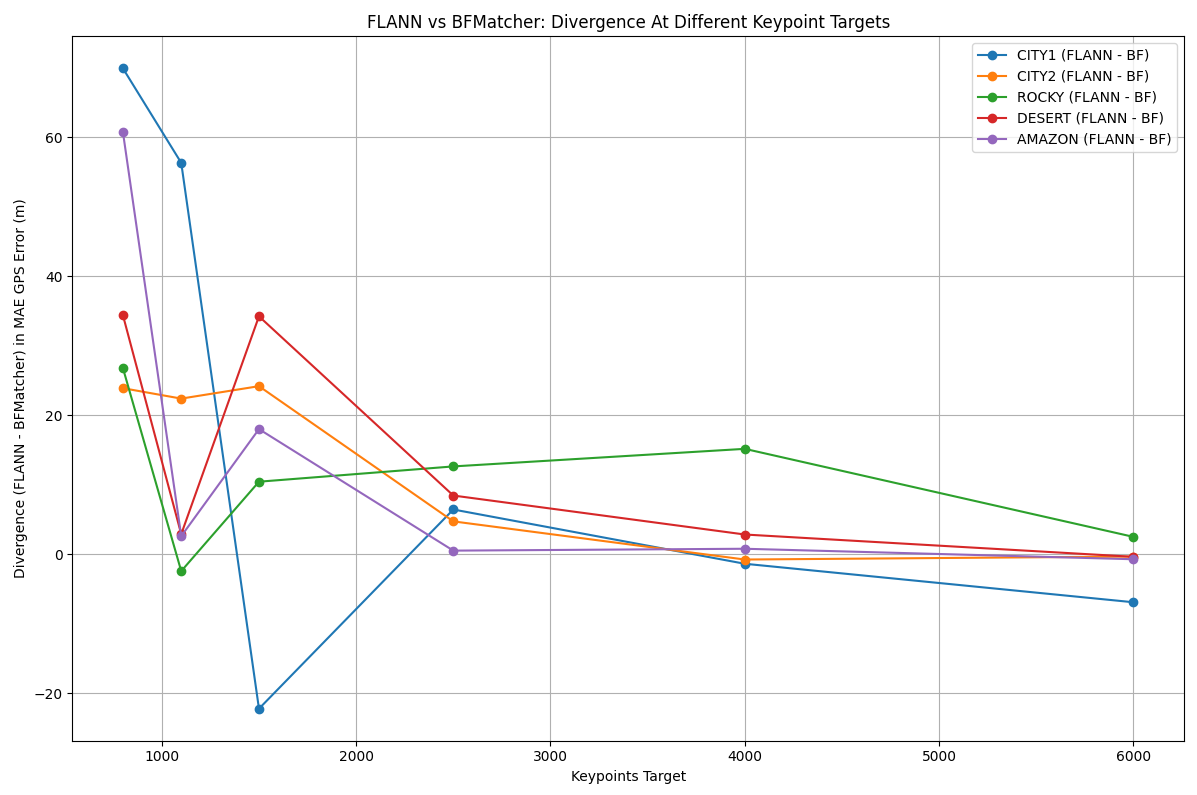
\includegraphics[width=\textwidth]{./Graphs/Divergence_BF_FLANN_KPS.png}
    \caption{Divergence in MAE GPS Error Between FLANN and BFMatcher Across Keypoint Targets.}
    \label{fig:divergence_plot}
\end{figure}

\textbf{Observations}

\begin{itemize}
    \item \textbf{Divergence and Convergence:}  
    As the number of keypoints increases, the difference in MAE GPS error between BFMatcher and FLANN decreases, showing that both matchers converge to similar levels of accuracy. At higher keypoint counts, the performance gap becomes negligible, with both methods providing comparable accuracy. Beyond 5000 keypoints, the error difference is minimal, well within acceptable limits for real-time applications.

    \item \textbf{Match Quantity vs Quality:}  
    Both matchers identified a similar number of matches in most tests, but the main distinction was in match quality. BFMatcher's exhaustive approach produced slightly higher-quality matches but required more processing time. FLANN, however, provided competitive accuracy with significantly faster runtimes, maintaining acceptable match quality.

    \item \textbf{Lowe's Ratio and Abnormalities:}  
    FLANN outperformed BFMatcher in several cases, primarily due to the effects of Lowe's filtering. Specifically:
    \begin{itemize}
        \item When Lowe's ratio was too lenient, incorrect matches could pass, but FLANN's approach often filtered these out by not identifying a suitable second match.
        \item When Lowe's ratio was too strict, valid matches could be discarded if the second-best match was too similar, but FLANN occasionally allowed these through by selecting slightly lower-quality second matches.
    \end{itemize}
    This demonstrates the limitations of static thresholds in Lowe's ratio and highlights the potential issues with overly rigid filtering.

    \item \textbf{Accuracy and Scalability:}  
    Both matchers showed decreasing error rates as the number of keypoints increased, improving overall stability. However, BFMatcher’s runtime increased much faster than FLANN's as the keypoint count grew, making FLANN a better option for handling larger datasets efficiently.

    \item \textbf{Implications:}  
    As keypoint counts rise, both matchers achieve comparable accuracy, but FLANN's superior efficiency and scalability make it the more practical choice for large-scale, real-time applications, balancing accuracy with computational cost.
\end{itemize}



\subsection*{4.3 Accuracy and Runtime Evaluation}

This evaluation compares the accuracy and runtime of BFMatcher and FLANN using optimized parameters for each dataset and matching method. The goal is to assess their trade-offs between precision and computational efficiency. Results are summarized in Table~\ref{tab:flann_bf_comparison}.

\begin{table}[H]
    \centering
    \begin{tabular}{|c|c|c|c|c|c|c|}
    \hline
    \makecell{\textbf{Matcher}} & 
    \makecell{\textbf{Metric Type}} & 
    \makecell{\textbf{CITY1}} & 
    \makecell{\textbf{CITY2}} & 
    \makecell{\textbf{ROCKY}} & 
    \makecell{\textbf{DESERT}} & 
    \makecell{\textbf{AMAZON}} \\
    \hline
    
    \multirow{2}{*}{\makecell{FLANN}} & 
    \makecell{MAE GPS \\ (m)} & 56.59 & 4.70 & 14.63 & 71.20 & 32.35 \\
    \cline{2-7}
    & \makecell{Runtime \\ (s)} & 42.72 & 41.61 & 41.96 & 43.42 & 53.62 \\
    \hline

    \multirow{2}{*}{\makecell{BF}} & 
    \makecell{MAE GPS \\ (m)} & 53.89 & 3.79 & 16.36 & 68.64 & 33.24 \\
    \cline{2-7}
    & \makecell{Runtime \\ (s)} & 203.49 & 228.59 & 46.33 & 52.59 & 88.95 \\
    \hline
    
    \end{tabular}
    \caption{Performance comparison of optimized BFMatcher and FLANN Across Datasets}
    \label{tab:flann_bf_comparison}
\end{table}

\textbf{Observations}
\begin{itemize}
    \item \textbf{BFMatcher} achieved slightly better MAE in some cases, but this precision came at the cost of significantly longer runtimes, with execution times often more than double those of FLANN.
    
    \item \textbf{FLANN} maintained faster runtimes across all datasets, demonstrating better computational efficiency, though with marginally higher MAE values in some scenarios.


    \item \textbf{Test conclusion:} FLANN is more suited for real-time applications, offering a practical balance between speed and accuracy, with scalability to handle larger datasets efficiently.
\end{itemize}




\section*{Conclusion} 
This study evaluated BFMatcher and FLANN for local feature matching. BFMatcher provided slightly higher-quality matches but was computationally expensive and more stable when fewer keypoints were available. FLANN, however, delivered comparable accuracy with significantly better runtime and scalability, making it ideal for real-time applications when sufficient keypoints are available.

In practice, with modern computational power generating high keypoint counts, the differences between the two methods become negligible. While BFMatcher shows more robustness under low-keypoint conditions, its lack of scalability makes it less practical compared to FLANN, which provides a more efficient solution without compromising accuracy.


\section*{Future Work} 
Future research should focus on: 
\begin{itemize} 
    \item \textbf{Adaptive Filtering:} Develop dynamic filtering techniques and inference models for determining optimal Lowe's threshold to address its limitations.  
    \item \textbf{Extreme Testing:} Explore the matchers' performance under more severe environmental conditions to improve robustness.  
    \item \textbf{Neural Network Integration:} Investigate ways to efficiently integrate learning-based matchers like LightGlue into real-time systems.
\end{itemize}

These improvements will enhance the robustness, efficiency, and applicability of feature matching in future systems.


\newpage
% The next critical feature in an image-based navigation system is the feature matcher. The feature matcher serves two main purposes. The first is to find the most highly correlated image pair. The second is to estimate the relative pose (translation and rotation) between the two images. Thus, we break up this section into two components, global matching and local matching. 
xxx check scale if or not if
To compute matches, The descriptor first transforms each feature individually to a normalized space. This process aligns the feature’s orientation, adjusts scale, and normalizes other factors like intensity, ensuring that each descriptor is in a consistent format for direct comparison during matching.


Matches have specific confidence levels. When calculating transformations we can include confidence weightings to improve the accuracy of the estimations. 

Broadly speaking there are two types of feature matchers: local and global. Local matchers are used to find the relative pose between two images. Global matchers are used to find the correlation between two images.

\section*{Local Matchers}
\subsection*{Brute-Force Matcher (BFMatcher)} BFMatcher compares every descriptor from one image with all descriptors in another image to find the closest match. It calculates the distance between descriptors using a chosen metric (e.g., Euclidean for SIFT, Hamming for ORB). Matches are sorted by distance, and the best ones are selected. While simple and effective, it can be slow with large datasets. Best suited for smaller datasets or when precision is prioritized over speed.

\subsection*{FLANN (Fast Library for Approximate Nearest Neighbors)} FLANN is an efficient matcher that uses approximate nearest neighbor search, speeding up the matching process, especially for large datasets. It uses tree-based algorithms or k-means clustering to quickly find matches. FLANN is often preferred for tasks involving large datasets where speed is critical, such as real-time applications with SIFT or SURF descriptors. FLANN must be used with Local-sensitivity hashing to allow for operations on its binary descriptors. 



\subsection*{Light Glue} Light Glue is a lightweight, relative to other neural network approaches, neural network-based matcher that uses deep learning to match features across images. It is optimized for speed and memory efficiency, making it suitable for mobile and embedded systems. Light Glue provides robust matches even under challenging conditions, such as significant viewpoint changes or lighting variations. This is a significant improvement over traditional feature matching methods like BF or FLANN matchers, however, it increases computational time and risks an inability to generalize well, especially in this context which is unlikely to have training data based off UAV images.

\section*{Improvements to Matching techniques}
\subsection*{Cross-Check Matching} Cross-check matching performs matching in both directions (from image A to B and B to A) and only retains matches that are consistent in both directions. This reduces false positives and increases the reliability of matches. However, this doubles the computation time.
 

\subsection*{RANSAC (Random Sample Consensus)} RANSAC is used to refine matches by identifying and removing outliers. It works by iteratively selecting a subset of matches, estimating a model (e.g., homography), and checking how well the remaining matches fit this model. Matches that deviate significantly are considered outliers and discarded. RANSAC is crucial in tasks like image stitching, where accurate geometric transformations are required.


\subsection*{SuperGlue} SuperGlue is a more advanced neural network-based matcher that leverages attention mechanisms, dynamically aggregating local features based on their inferred importance, to enhance the matching process. It works by learning to match keypoints directly from image data, providing superior performance in complex scenarios with large changes in scale, rotation, or perspective. SuperGlue is well-suited for high-precision applications like 3D reconstruction. 


\section*{Global Matchers}

Global matchers aim to capture the overall similarity between images. Many techniques, like local matchers, do not inherently test similarity evenly across the image and therefore may tend to compare local zones instead of the entire context. This leads to sub-par matching and pose inference. 
To ensure full context, we can either choose a global matcher that already considers the entire image space, or use one that does not and divide into grids and compare per-grid to ensure complete context. In both cases, the scale and rotation should be normalized between images unless explicitly invariant to these. 
The following are chosen based on their ability to be computationally efficient and not require any pre- or live-training.

\subsection*{Translation affects the results of these}

\subsection*{Local matching conversion techniques}
These are techniques which convert local matchers, which are translation invariant, into techniques which penalize translation in its score. From the above local matchers, tests will be conducted on 

\subsection*{Histograms}

\subsection*{Hashing Methods}  
Hashing methods, like LSH (Local-sensitivity hashing) or PCA (Principal-component analysis), map high-dimensional descriptors to a lower-dimensional space. Hashing focuses on descriptor similarity rather than relative spatial positions within the image. Grid-rot apply

\subsection*{SSIM (Structural Similarity Index)}  
SSIM compares images based on luminance, contrast, and structural information, making it sensitive to spatial shifts like translation. 

\subsection*{KNN or other local Matching}  
Adapting local matchers, such as AKAZE, for global matching allows for high accuracy. 

Use low threshold, per-grid matching, and count the amount of matches. This is point-to-point and can be computationally expensive when comparing many images. 



\subsubsection*{Plan}
These methods offer complex tradeoffs within different accuracy and speed metrics. As such, tests will be conducted on individual methods as well as hybrid approaches. All of the above methods will be included in these tests except the deep-learning approaches which are too computationally intensive for the task of finding the most correlated image. The best method is that which results in the combination of image pairs (matches) which subtends the lowest mean squared deviation in actual and estimated GPS locations and heading. 


To summarize: the invariant methods are: Hashing, BOVW; variant methods are 



Intermediary results:

These results indicate the time to complete the set of best correlated images. The score has not been used as the highly variant parameter set often, with enough computation, can achieve the correct score. So instead of holding computational time constant, which is not clear, we increase the parameters until we see it achieve the correct score. Then the time is recorded and a higher accuracy is dually implied in a lower time. Where excessive time is required and the correct combination has not been met, there will be an indication of failure to meet score. 
Excessive time is defined as greater than 10s for an image space of 12. 

\begin{table}[H]
    \centering
    \begin{tabular}{|c|c|}
    \hline
    \textbf{Search Space (Images)} & \textbf{Runtime (Seconds)} \\ \hline
    12  & 5.04 \\ \hline
    11  & 5.14 \\ \hline
    10  & 4.90 \\ \hline
    9   & 4.30 \\ \hline
    8   & 3.74 \\ \hline
    7   & 3.56 \\ \hline
    6   & 3.12 \\ \hline
    5   & 2.59 \\ \hline
    4   & 1.99 \\ \hline
    3   & 1.51 \\ \hline
    2   & 0.98 \\ \hline
    1   & 0.49 \\ \hline
    \end{tabular}
    \caption{KNN Matching: Search Space vs. Runtime}
    \end{table}

For BF_matching with KNN search, the run-time per image is roughly half a second, and the time complexity is linear.   

% \section*{Concept}

The flow of the camera system shall be as follows:

\begin{enumerate}
    \item The controller shall receive footage in real-time from the UAV and sync it with known telemetry data such as GPS coordinates, altitude, heading and speed.
    \item The controller shall then process the video footage and telemetry data to extract and store the relevant features
    \item When the GPS signal is lost, the UAV will turn around
    \item The controller shall extract and match the features of the current image with that of the previous images
    \item It will find the most correlated images and use that image to determine the change in feature locations to infer the UAV's position
\end{enumerate}




XXX - flat earth buildings assumption
XXX - try 512 x 512
XXX - different datasets


\section{Rotational Estimators}

\subsection{Introduction}
Rotational estimators are critical in image alignment and pose estimation tasks. In this project, rotational estimators are employed to align UAV-captured images when GPS data is unreliable. The accuracy of rotational alignment directly impacts the estimation of translational shifts and image similarity. These steps are crucial to ensuring reliable navigation in GPS-denied environments.

Four methods were selected for rotational estimation based on their applicability, computational efficiency, and accuracy. Other methods were considered but ultimately excluded due to their efficiency or accuracy.   

\subsection{Methods}
\begin{itemize}
    \item \textbf{Homography Estimation}: A method supporting 8 degrees of freedom (DoF), accounting for rotation, scaling, translation, and perspective correction. It is suitable for complex transformations but may introduce unnecessary errors when perspective correction is not needed.
    \item \textbf{Affine Estimation}: A method with 6 degrees of freedom that handles rotation, scaling, and translation without perspective correction. It is computationally efficient and offers sufficient transformation handling for most tasks.
    \item \textbf{2x2 Rotation Matrix}: A simplified method that accounts only for rotational and translational freedom. It lacks support for scaling and perspective, making it less effective for complex transformations.
    \item \textbf{Vector-based Estimation}: A direct estimation of rotation using vectors derived from image points. This method lacks robust outlier removal and complexity, limiting its effectiveness for real-world applications.
\end{itemize}

\textbf{Conclusion:} These methods were chosen to provide a range of complexity and computational efficiency, with homography and affine estimation being the primary focus due to their broader applicability in image transformations.

\subsection{Improvement Techniques}
To enhance the accuracy and robustness of these methods, the following improvement techniques were applied:
\begin{itemize}
    \item \textbf{Lowe's Ratio with KNN}: Filters out ambiguous matches by comparing the best match with the second-best match, effectively eliminating outliers, especially in repetitive or noisy data.
    \item \textbf{RANSAC (Random Sample Consensus)}: A robust outlier removal technique that iteratively refines the inlier set to accurately estimate transformations.
    \item \textbf{Confidence Thresholds}: Filters out matches or keypoints below a certain confidence level. In practice, this technique performed worse than Lowe's Ratio and RANSAC, and when used alongside them, it reduced accuracy due to over-filtering.
    \item \textbf{Confidence Weightings}: Adjusts the influence of each match based on its confidence score. Similar to confidence thresholds, this technique led to decreased stability by over-filtering.
\end{itemize}

\textbf{Conclusion:} The combination of Lowe's Ratio and RANSAC was the most effective in improving accuracy and robustness. Confidence thresholds and weightings were found to be redundant.

\subsection{Initial Accuracy Testing}
Initial tests were conducted using relatively optimal parameters, and the performance of each method was evaluated based on its Mean Absolute Error (MAE) in heading relative to the ground truth. The results are summarized below:

\begin{table}[H]
    \centering
    \begin{tabular}{|c|c|c|}
        \hline
        \textbf{Method} & \textbf{MAE (heading)} & \textbf{Result} \\
        \hline
        Homography & 0.1207 & Accurate \\  
        Affine & 0.1129 & Best-performing \\  
        2x2 Rotation Matrix & 1.0277 & Poor performance \\  
        Vector-based & 7.3571 & Poor performance \\  
        \hline
    \end{tabular}
    \caption{Initial Testing Results (MAE - Mean Absolute GPS Error)}
\end{table}

\textbf{Conclusion:} The affine method achieved the lowest MAE, making it the most accurate for aligning images. Homography performed slightly worse due to its additional degrees of freedom, which introduced unnecessary errors. The 2x2 rotation matrix and vector-based methods were unsuitable for the task due to their lack of transformation handling complexity. Based on these results, affine and homography were selected for further testing.

\subsection{Accuracy in Global and Local Matching}
To assess the overall suitability of the rotational estimators, it is crucial to evaluate their impact on the system as a whole. Focusing solely on heading errors does not capture the full extent of how minor inaccuracies propagate through the system. By examining the Mean Normalized Error (MNE) in GPS coordinates, a more realistic understanding of the cumulative effect of small rotational errors and their influence on overall system performance is obtained.

\begin{table}[H]
    \centering
    \begin{tabular}{|c|c|c|}
        \hline
        \textbf{Global Method} & \textbf{Local Method} & \textbf{Mean Normalized Error (GPS)} \\  
        \hline
        Homography & Homography & 48.90 \\  
        Homography & Affine & 41.80 \\  
        Affine & Homography & 42.37 \\  
        Affine & Affine & 41.28 \\  
        \hline
    \end{tabular}
    \caption{Accuracy Comparison for Global and Local Matching Techniques (MNE - Mean Normalized Error)}
\end{table}

\textbf{Conclusion:} The affine method consistently outperforms homography in both global and local matching scenarios. The significant reductions in GPS error, even with relatively minor decreases in rotational error, highlight the sensitivity of both methods to rotational inaccuracies. This underscores the critical importance of optimizing the accuracy of the rotational stage.


\subsection{Time Constraints}
Time efficiency was evaluated to assess the computational performance of each method. The table below summarizes the average, minimum, median, and maximum runtimes for each approach. Lower computation times enable higher frame rates, provide greater tolerance for minor errors, and allow for faster processing of larger search spaces, ultimately improving accuracy.


\begin{table}[H]
    \centering
    \begin{tabular}{|c|c|c|c|c|}
        \hline
        \textbf{Method} & \makecell{\textbf{Mean Time} \\ \textbf{(ms)}} & \makecell{\textbf{Max Time} \\ \textbf{(ms)}} & \makecell{\textbf{Min Time} \\ \textbf{(ms)}} & \makecell{\textbf{Median Time} \\ \textbf{(ms)}} \\
        \hline
        Affine & 1.276 & 11.55 & 0.00 & 0.999 \\  
        Homography & 22.58 & 50.74 & 0.98 & 10.80 \\  
        \hline
    \end{tabular}
    \caption{Time Analysis for Affine and Homography Methods}
\end{table}

\textbf{Conclusion:} Affine is significantly faster than homography, with a much lower mean and median runtime. The greater variability in homography’s runtime (indicated by the difference between mean and median) is due to its handling of more complex transformations. Affine’s speed makes it particularly well-suited for real-time UAV applications.

\subsection{Robustness Testing}
Robustness testing was performed to assess each method's sensitivity to different parameter settings, such as RANSAC thresholds, Lowe’s ratio for match filtering, and keypoint confidence thresholds. These tests are essential to determine the methods’ reliability under varying conditions and data quality.

\subsubsection{RANSAC Threshold Testing}
We varied RANSAC thresholds to evaluate how sensitive each method is to outlier removal. A lower threshold implies more aggressive filtering, which reduces the number of keypoints but increases the reliability of those retained.

\begin{table}[H]
    \centering
    \begin{tabular}{|c|c|c|}
        \hline
        \textbf{Threshold} & \makecell{\textbf{Homography (Mean} \\ \textbf{Heading Error)}} & \makecell{\textbf{Affine (Mean} \\ \textbf{Heading Error)}} \\
        \hline
        0.2 & 0.1384 & 0.1089 \\  
        0.5 (Default) & 0.1207 & 0.1129 \\  
        5 & 0.1249 & 0.1003 \\  
        25 & 0.1222 & 0.0997 \\  
        50 & 0.1226 & 0.1112 \\  
        \hline
    \end{tabular}
    \caption{Effect of RANSAC Thresholds on Heading Error}
\end{table}

\textbf{Conclusion:} Both methods are robust to RANSAC threshold changes, but homography exhibits greater variability at lower thresholds, suggesting a weaker estimation capability when fewer keypoints are available.

\subsubsection{Lowe's Ratio Testing}
We evaluated Lowe's ratio to assess its impact on match filtering and rotational estimation accuracy. A lower ratio implies more aggressive filtering, reducing the number of matches but increasing their quality.

\begin{table}[H]
    \centering
    \begin{tabular}{|c|c|c|}
        \hline
        \textbf{Lowe's Ratio} & \makecell{\textbf{Homography (Mean} \\ \textbf{Heading Error)}} & \makecell{\textbf{Affine (Mean} \\ \textbf{Heading Error)}} \\
        \hline
        0.6 & 0.1289 & 0.1098 \\  
        0.7 & 0.1255 & 0.1006 \\  
        0.8 & 0.1207 & 0.0997 \\  
        0.9 & 0.1139 & 0.1111 \\  
        0.95 & 0.1211 & 0.1054 \\  
        \hline
    \end{tabular}
    \caption{Effect of Lowe's Ratio on Heading Error}
\end{table}

\textbf{Conclusion:} Both methods are robust to changes in Lowe’s ratio. 

\subsubsection{Keypoint Confidence Threshold Testing}
Keypoint confidence thresholds were varied to evaluate how each method performs with different levels of keypoint quality. Lower thresholds admit more keypoints but decrease the reliability of individual keypoints.

\begin{table}[H]
    \centering
    \begin{tabular}{|c|c|c|}
        \hline
        \makecell{\textbf{Keypoint Confidence} \\ \textbf{Threshold}} & \makecell{\textbf{Homography (Mean} \\ \textbf{Heading Error)}} & \makecell{\textbf{Affine (Mean} \\ \textbf{Heading Error)}}\\
        \hline
        0.001 & 0.1404 & 0.1019 \\  
        0.0008 & 0.1207 & 0.0974 \\  
        0.0005 & 0.1247 & 0.0997 \\  
        0.0002 & 0.1247 & 0.1024 \\  
        \hline
    \end{tabular}
    \caption{Effect of Keypoint Confidence Thresholds on Heading Error}
\end{table}

\textbf{Conclusion:} Both methods are robust to changes in keypoint confidence thresholds, but affine remains more consistent at lower thresholds, maintaining lower mean errors with noisier keypoints.

\subsubsection{Overall Robustness}
In summary, affine consistently outperforms homography in terms of robustness, particularly in scenarios involving noisier or fewer keypoints. This makes affine the preferred method for handling datasets with varying quality and practical applications requiring stability under changing conditions.

\subsection{Conclusion}
Affine estimation is selected as the primary method for future work due to its superior accuracy, faster computation, and greater robustness. Its 6 degrees of freedom provide sufficient understanding of image transformations without introducing unnecessary errors from perspective correction. 


Best Rotator: Affine, AKAZE AND BF




\subsection*{Matching filtration techniques}
Global point matching. In order to find an accurate rotational estimate, we need to ensure that the points we use in the inference are of sufficient quality and quantity. This involves filtering out lower quality keypoints while considering sufficient keypoints are still needed to remove noise from resolution and computation limits and distortion-based point differences. This means we need to filter the matches between images. The first is to remove ambiguous matches. This involves using Lowes Ratio's Test to ensure the two best potential matches are sufficiently different based on their descriptors. Then, we can sort the matches according to how close the match is to its actual corresponding keypoint based on their descriptors. Finally, we can use homography and RANSAC to firstly estimate a model for the data points and reject any outliers to this model. Together, these steps remove ambiguity, ensure matches are of high quality, and remove outliers to ensure the best possible rotational estimate.
The three parameters associated with each of these steps are:
\begin{itemize}
    \item \textbf{Lowes Ratio Test}: This is the ratio of the distance of the best match to the second-best match. If this ratio is above a certain similarity allowed threshold, the match is considered ambiguous and removed. 
    \item \textbf{Homography and RANSAC}: The homography and RANSAC model is used to estimate the transformation between the two images. The RANSAC threshold is the maximum distance a point can be from the model to be considered an inlier. 
    \item \textbf{Keypoint Confidence Threshold}: This is the minimum confidence a keypoint must have to be considered in the matching process. This may be only keeping some number of the highest quality keypoints or keeping all keypoints above a certain similarity threshold. The former will be used as this ensures that we do not have to constantly adjust the threshold based on the dataset and quality, instead we are guaranteed to have a certain number of keypoints which is more important than being pedantic about the quality of the keypoints.
\end{itemize}
    
Note, this is tested on only the global matcher, and with multimethod, implying isolation in its effect on the rotational estimation. XXX this still now needs to be tested with the global matcher being the local matcher (added inferred effect) and on the local matcher. 
    Testing Kp threshold confidences:



    
AKAZE NO FILTER:
Percentage Deviation: [4.91698283] %
Preprocessing Global Detector: AKAZE, Preprocessing Global Matcher: BF, Global Matching Technique: Histogram, Local Detector: AKAZE, Local Matcher: BF
Mean normalized GPS error: [65.07094916]
 Mean Heading Error: 0.8556339319426911
Mean Length of Keypoints: 2525.866666666667
Mean Global Time to Extract Keypoints: 0.2709 s
Mean Number of Good Matches: 802.4396551724138
Range of Good Matches: 1524
Time taken to execute The Method: 45.7884 seconds

AKAZE 500
Percentage Deviation: [4.58746506] %
Preprocessing Global Detector: AKAZE, Preprocessing Global Matcher: BF, Global Matching Technique: Histogram, Local Detector: AKAZE, Local Matcher: BF
Mean normalized GPS error: [62.34674896]
 Mean Heading Error: 0.9235667588307905
Mean Length of Keypoints: 2525.866666666667
Mean Global Time to Extract Keypoints: 0.4008 s
Mean Number of Good Matches: 500.0
Range of Good Matches: 1524
Time taken to execute The Method: 62.8682 seconds



AKAZZE 300
Percentage Deviation: [4.53573965] %
Preprocessing Global Detector: AKAZE, Preprocessing Global Matcher: BF, Global Matching Technique: Histogram, Local Detector: AKAZE, Local Matcher: BF
Mean normalized GPS error: [61.64376568]
 Mean Heading Error: 0.9238056255750251
Mean Length of Keypoints: 2525.866666666667
Mean Global Time to Extract Keypoints: 0.2578 s
Mean Number of Good Matches: 300.0
Range of Good Matches: 1524
Time taken to execute The Method: 45.2109 seconds



\begin{table}[H]
    \centering
    \begin{tabular}{|c|c|c|c|c|c|c|}
        \hline
        \makecell{\textbf{Keypoints} \\ \textbf{Allowed}} & \textbf{No Filter} & \textbf{500} & \textbf{300} & \textbf{No Filter} & \textbf{500} & \textbf{300} \\ 
        \hline
        \multicolumn{1}{|c|}{\textbf{Method}} & \multicolumn{3}{c|}{\textbf{AKAZE}} & \multicolumn{3}{c|}{\textbf{ORB}} \\
        \hline
        \makecell{\textbf{GPS Error}} & 65.07 & 62.35 & 61.64 & 54.10 & 56.72 & 60.64 \\  
        \hline
        \makecell{\textbf{Mean Number} \\ \textbf{of Good Matches}} & 802.44 & 500.0 & 300.0 & 718.15 & 500.0 & 300.0 \\  
        \hline
        \makecell{\textbf{Range of} \\ \textbf{Good Matches}} & 1524 & 1524 & 1524 & 0 & 0 & 0 \\  
        \hline
        \makecell{\textbf{Mean Length} \\ \textbf{of Keypoints}} & 2525.87 & 2525.87 & 2525.87 & 3000.0 & 3000.0 & 3000.0 \\  
        \hline
        \makecell{\textbf{Time Per Keypoint} \\ \textbf{Extraction (s)}} & 0.2709 & 0.4008 & 0.2578 & 0.0636 & 0.0916 & 0.0571 \\  
        \hline
        \makecell{\textbf{Time Taken} \\ \textbf{(seconds)}} & 45.79 & 62.87 & 45.21 & 48.08 &  47.3382 & 46.04 \\  
        \hline
    \end{tabular}
    \caption{Comparison of AKAZE and ORB Feature Matching Performance}
\end{table}




From this table, its clear the optimal point for ORB is without filtering the matches given that ORB was running with only 3000 keypoints. For AKAZE, this point is at 300. This optimal point is based mainly on accuracy with consideration for no large time difference. As visible, ORB outperforms AKAZE in accuracy given roughly similar time constraints. 


As visible, ORB outperforms AKAZE in accuracy given roughly similar time constraints. The time is also more consistent accross different datasets implying more robustness. 
\graphicspath{{conclusion/fig/}}

\chapter{Summary and Conclusion}
\label{chap:conclusion}



% Bibliography
\bibliography{mybib}

% End matter
\appendix
\chapter{Project Planning Schedule}
\makeatletter\@mkboth{}{Appendix}\makeatother
\label{appen:derivations_bigramseg}

This is an appendix.

\chapter{Outcomes Compliance}
\makeatletter\@mkboth{}{Appendix}\makeatother
\label{appen:derivations_bigramseg}

This is another appendix.

\end{document}

